\documentclass[a4print,english,lof,lot,twoside]{univpmthesis}
\errorcontextlines=9

\RequirePackage[utf8]{inputenc}
\RequirePackage[T1]{fontenc}

\usepackage{lmodern}

%%%%%%%%%%%%%%%%%%%%%%%%%%%%%%%%%%%%%%%%%%%%%%%%%%%%%%%%%%%
% Metadata
%%%%%%%%%%%%%%%%%%%%%%%%%%%%%%%%%%%%%%%%%%%%%%%%%%%%%%%%%%%
\thfaculty{\textbf{Facolt\`{a} di Ingegneria}}
\thcourse{\textbf{Corso di Laurea in Ingegneria Informatica e dell'Automazione}}

\thtitle{Diagnosi di tumori cutanei tramite reti neurali pre-addestrate nel framework \textit{concept-bottleneck models}} 
\thsubtitle{Skin cancer diagnosis using pre-trained neural networks in the concept-bottleneck models framework}

%\thsubtitle{Sottotitolo della Tesi} % NON NECESSARIO
\thauthor{Camilloni Andrea}
\thadvisor{Prof.~Simone Fiori}
\thcoadvisor{Dr.~Hwee Kuan Lee\\}{Dr.~Davide Coppola}{}


\ayear{\textbf{2020-2021}}
\thesisdedication{I put my heart and soul into my work, and I have lost my mind in the process.\\ Vincent Willem van Gogh}
\thlocation{Ancona}
\thtime{Luglio 2021} % data scrittura
%%%%%%%%%%%%%%%%%%%%%%%%%%%%%%%%%%%%%%%%%%%%%%%%%%%%%%%%%%%

\usepackage{amsmath,amsfonts,amssymb,bm} %<- scrittura equazioni
\usepackage[italian,english]{babel}
\usepackage{graphicx,subcaption} 	%<- immagini
\usepackage{epstopdf} 	%<- conversione immagini .eps
	%<- sottofigure
\usepackage{footnote}	%<- note a piè pagina
\usepackage{tabularx,booktabs,multicol,multirow} %<- tabelle
\usepackage{mathrsfs}
\usepackage{caption}	%<- didascalie
\usepackage{microtype}
\usepackage{gensymb,siunitx}	%<- simboli ed unità di misura
\usepackage{hyperref}
\usepackage{glossaries}
\usepackage{verbatim}
\usepackage{xcolor}
\usepackage[a-1b]{pdfx} %<- generazione pdf-A
\usepackage{enumitem} %per liste
\newcommand{\R}{\mathbb{R}}
% Solo per generare testo, da cancellare quando si inizia a scrivere:
\usepackage{lipsum}
    \newlength{\itemizewidth}% <-- text width in itemize
    \setlength{\itemizewidth}{\dimexpr\linewidth-\leftmargini\relax}

\usepackage{rotating}
\usepackage{pdflscape}
%%%%%%%%%%%%%%%%%%%%%%%%%%%%%%%%%%%%%%%%%%%%%%%%%%%%%%%%%%%
\newcommand{\eqname}{Eq.}
%%%%%%%%%%%%%%%%%%%%%%%%%%%%%%%%%%%%%%%%%%%%%%%%%%%%%%%%%%%

\begin{document}

 

%%%%%%%%%%%%%%%%%%%%%%%%%%%%%%%%%%%%%%%%%%%%%%%%%%%%%%%%%%%
% Front matter contents
%%%%%%%%%%%%%%%%%%%%%%%%%%%%%%%%%%%%%%%%%%%%%%%%%%%%%%%%%%%
\frontmatter

\maketitle

\begin{thesisacknowledge}[italian]Un particolare ringraziamento va al prof. Fiori, sempre disponibile e paziente, il quale mi ha dato la possibilità di effettuare un tirocinio "fuori dagli schemi". \\
Un sentito grazie al Dott. Davide Coppola, correlatore di tesi, per il supporto costante, le dritte indispensabili e la sua complicità nella realizzazione della mia tesi, e al Dott. Hwee Kuan Lee, per avermi dato la possibilità di entrare a far parte del suo team di ricerca.\\
Ai miei professori del corso di studi, che in un modo o nell'altro hanno contribuito a dare forma al futuro ingegnere che è in me, e senza i quali non avrei raggiunto il tanto atteso traguardo che oggi celebro.\\
Ai miei genitori, che in questi anni mi hanno sopportato, sostenendomi sempre e appoggiando ogni mia decisione. \\
A mia sorella Sofia, sempre al mio fianco in questo percorso. \\
Ai miei amici, per esserci sempre stati. \\
Desidero infine ringraziare il mio allenatore Maykol, per avermi guidato in questi anni e insegnato a non mollare mai.
\end{thesisacknowledge}
\begin{thesisabstract}[english]
Deep learning techniques have been widely used in the medical field for image classification and in the past few years have shown to be successful in providing good diagnostic accuracy.\\
Skin cancer is a common and deadly disease that a Deep Convolutional Neural Network(CNN) could detect. Clinical images and images acquired by using a particular handheld instrument , called Dermatoscope, could be used in order to provide a diagnosis. 
To study this possibility, a few datasets have been released over the years. This work focuses on the Derm7pt dataset, which provides labels for 7 clinically significant attributes in addition to the diagnosis of the lesion. These attributes are part of the 7-point checklist method used in clinical practice.
The goal of this thesis is to provide a model able to detect Melanoma in dermoscopic images of skin lesions, by learning first a set of human-understandable concepts.
To do this, the Concept Bottleneck Framework was employed, by designing models that first predict the clinical attributes from 7-point checklist method and then use those for the final diagnosis of the lesion.
These models have then been compared with the more widespread Single Task Learning approaches, which learn the diagnosis end-to-end without intermediate concepts.\\
The bottleneck model that showed the best performance in melanoma diagnosis achieved an accuracy and F1 score of $77.50\%$, and $65.60\%$ respectively.
The Single Task Learning approach obtained the best result by achieving an accuracy and F1 score of $81.25\%$, and $67.96\%$. \\
The experiments have shown that the performance of the black-box models is slightly superior. However, they lose the ability to provide further insights into prediction as Concepts Bottleneck Models can do. \\


\end{thesisabstract}

\begin{thesisabstract}[italian]
Le tecniche di deep learning sono state ampiamente utilizzate in campo medico per la classificazione delle immagini e negli ultimi anni hanno dimostrato di essere efficaci nel fornire una buona accuratezza diagnostica. \\
Il tumore della pelle, identificato in alcune forme come Melanoma, è una causa comune di morte nella popolazione odierna, se non diagnosticato precocemente; le reti neurali convoluzionali profonde, o CNN, possono rilevarlo a partire da una semplice immagine. 
Immagini acquisite clinicamente, o tramite appositi strumenti, come ad esempio il Dermatoscopio, il quale mette in evidenza pattern non visibili ad occhio nudo di una lesione cutanea, possono esser analizzate da una CNN per fornire una diagnosi precoce.\\
Negli anni, alcuni dataset sono stati resi disponibili per dare la possibilità di approfondire la materia.\\
In questo lavoro, è stato usato il dataset Derm7pt, il quale fornisce le labels per 7 importanti attributi clinici, in aggiunta alla diagnosi della  relativa lesione cutanea. Questi attributi sono la caratteristica principale del metodo di classificazione, usato in ambiente clinico dai dermatologi, conosciuto come \textit{7-point checklist}.
Questa tesi propone diversi metodi per classificare una lesione cutanea, differenziandola tra Melanoma e Nevi.\\
Un grande ostacolo incontrato nei metodi proposti nella letteratura è quello rappresentato dalla natura delle reti neurali, le quali sono delle “scatole chiuse”, che non forniscono un’ interpretazione umana di come hanno effettuato le loro predizioni. Quindi un particolare focus, nel lavoro proposto, è andato ad architetture conosciute come Concept Bottleneck Models(CBM), le quali apprendono un set di concetti intermedi (i 7 attributi del 7-pt Checklist), interpretabili dall’umano e fanno infine la predizione sulla diagnosi.\\
Sono state poi confrontate le diverse architetture basate sul framework dei Concept Bottleneck Models con architetture end-to-end, cioè delle scatole chiuse che predicono direttamente la diagnosi.\\
Gli esperimenti hanno mostrato i migliori risultati sulla diagnosi finale, ottenuti dai modelli end-to-end, seppur perdendo l’abilità di fornire una spiegazione della predizione, come i CBM possono fare.\\
In particolare, la miglior accuratezza nella predizione è stata fornita dal modello costituito da una ResidualNet pre-addestrata, i cui layer finali sono stati addestrati nuovamente su un test set del dataset proposto, ottenendo circa un'accuratezza del $81.25\%$, e un F1 score del $67.96\%$.\\
Mentre l'implementazione nel framework CBM, che ha ottenuto la miglior performance è stata l'archittettura Sequential, nella quale addestrando prima la base del modello costituita da un InceptionNet per predire i concetti e, allenando successivamente la testa del modello con i concetti predetti, ha ottenuto rispettivamente un'accuratezza e un F1 score del $77.50\%$ e $65.60\%$. \\
Nel complesso le architetture proposte hanno comunque ottenuto buoni risultati, comparabili con le regole, come ad esempio la 7-point Checklist Rule, proposte nella letteratura. Applicando infatti la precedente regola sui concetti reali, sono stati ottenuti i seguenti risultati $83.44\%$ e $78.43\%$ rispettivamente per le 2 metriche. \\

\end{thesisabstract}


\thesistoc

%%%%%%%%%%%%%%%%%%%%%%%%%%%%%%%%%%%%%%%%%%%%%%%%%%%%%%%%%%%
% Main matter contents
%%%%%%%%%%%%%%%%%%%%%%%%%%%%%%%%%%%%%%%%%%%%%%%%%%%%%%%%%%%
\mainmatter

\graphicspath{{chapters/chapter1/}}
\chapter{Introduction} \label{introduction}
Skin cancer is the most common malignancy in fairskinned populations, and the incidences of melanoma and non-melanoma skin cancers have been rising in recent years~\cite{7ptCNNforMel}. If undetected these malignancies have high death rate, but early diagnosis of melanoma has been shown to reverse the odds in the majority of cases~\cite{mtl7ptCoppola}. \\
Skin cancer detection seems to be accurate when performed by dermatologist using a dermatoscope, which is a handheld instrument that permits in vivo evaluation of colors and microstructures of the skin that are not visible to the naked eye. In the literature some algorithms for melanoma diagnosis have been studied, and one of them is the 7 point checklist \cite{Kawahara}, which consists in looking for irregular patterns and assigning a score to them: melanoma is diagnosed if a score greater or equal than 3 is achieved~\cite{Kawahara}. \\
Deep learning methods show great performance in melanoma diagnosis and they could be an important tool in medical applications. However, in a real-world scenario, an interpretation of how the model predict the diagnosis, is a need for dermatologists to be sure about the final diagnosis; most state-of-the-art models today do not typically give an explanation about theirs predictions, because they are end-to-end models that go from raw input $x$(e.g. image) to target $y$(e.g. melanoma diagnosis).\\
So in this work, several implementations of end-to-end models were compared with concept bottleneck models(CBM)\cite{CBM} for prediction of melanoma diagnosis in skin lesion images. \\
CBM allow to approach the problem of explaining how the model makes its predictions by revisiting the idea of first predicting an intermediate set of human-specified concepts like "atypical pigment network", then using them to predict the target $y$(Melanoma or Nevus). \\
In this work, experiments were carried out on different approaches, from the most widespread,the Single Task Learning, to the implementation of CBMs.
In the case of Single Task Learning, different methods were presented, based on the use of pre-trained networks, respectively InceptionV3\cite{IncNet} and ResNet101V2\cite{Resnet}; furthermore, the performance of these models was tested both by freezing the pre-trained weights and fine-tuning them to the problem at hand.
With regard to the CBM implementations, pre-trained Multi Task Learning architectures have been used as intermediate models for the concepts prediction; whereas logistic regression model was used for the final classification. For these experiments, the independent and sequential configurations described in \cite{CBM} have been implemented.\\
This manuscript begins with a brief overview of medical and technical background, followed by proposed works in the literature that deal with automated diagnosis of skin lesions. This is followed by a description of the 7-point derm dataset and the methods that have been used for the experiments. The last chapters presents the experimental setups and results obtained in the experiments as well as a conclusion to the work.



\graphicspath{{chapters/chapter2/}}
\chapter{State of the Art} \label{chapter2}
\section{Medical background}
\label{7ptSection}
%%%
\subsection{Skin Lesion}
A \textbf{skin lesion} is a part of the skin that has particular differences from the surrounding skin; the American Society for Dermatologic Surgery described it as an abnormal lump, bump, ulcer, sore, or colored area of the skin.
There are different types of skin lesion which differ in their characteristics such as shape, surface, colour, structure which could change overtime (See Figures \ref{fig:MEL_images} and \ref{fig:NEV_images} for an example) \\
Figure~\ref{fig:NEV_images} shows one of the most common skin lesions in the population, a Nevus. \textbf{Nevus}, also called mole, is a growth on the skin that develops when pigment cells (melanocytes) grow in clusters.  Nevus is harmless, and rarely can turn into skin cancer. \\
Skin lesions can be temporary or permanent depending on the causes, and most of them, as nevi, are harmless, but some can be warnings of skin cancer.\\
Skin cancer is the most common malignancy in fairskinned populations, and the incidences of melanoma and non-melanoma skin cancers are rising \cite{7ptCNNforMel}.
There are three common types of skin cancers: squamous cell carcinoma(SCC), basal cell carcinoma(BCC) and \textbf{melanoma}. The first two are tipically grouped together as non melanoma skin cancer, while malignant Melanoma (Figure~\ref{fig:MEL_images}) is a type of skin cancer which tends to spread to the other parts of the body causing death if is not diagnosed early \cite{7ptCNNforMel}\\
Early melanoma diagnosis showed to reverse the odds in the majority of cases \cite{mtl7ptCoppola}.
Wrong diagnosis  could cause death, especially when melanomas have a non-alarming clinical appearance and imitate a completely benign lesion. Against that, dermatologists nowadays are adopting innovative tools such as the dermatoscope for the acquisition of clearer images for an accurate diagnosis. Such tools along with particular rules and methods have allowed efficient identification of the early phase of cutaneous malignant melanoma.\\

\begin{figure}
    \centering
    \begin{subfigure}[b]{0.48\linewidth}        %% or \columnwidth
        \centering
        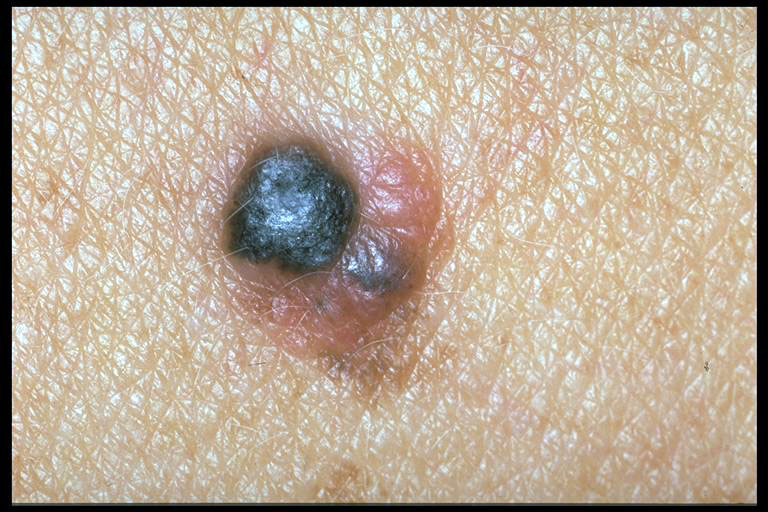
\includegraphics[width=\linewidth]{images/skin lesion/MEL/Gcl051.jpg}
        \caption{Clinical image\footnotemark[1]}
        
        \label{fig:Mel_A}
    \end{subfigure}
    \begin{subfigure}[b]{0.48\linewidth}        %% or \columnwidth
        \centering
        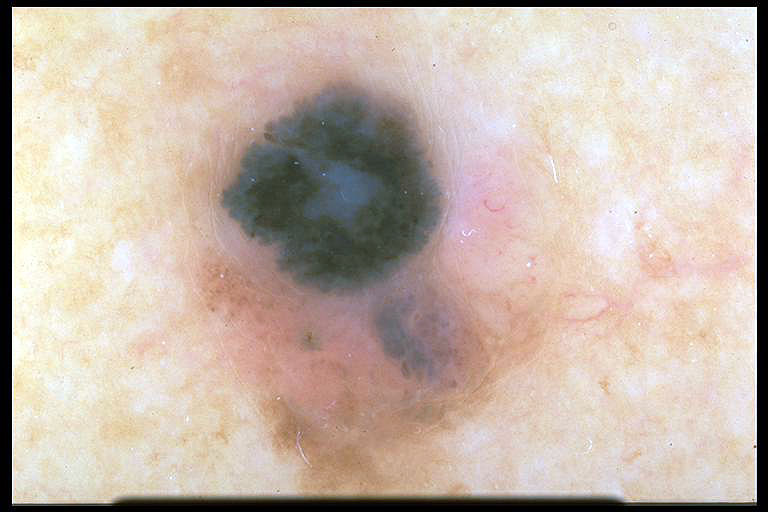
\includegraphics[width=\linewidth]{images/skin lesion/MEL/Gcl052.jpg}
        \caption{Dermatoscopy image\footnotemark[2]}
        \label{fig:Mel_B}
    \end{subfigure}
    \caption*{Source: https://derm.cs.sfu.ca/Welcome.html}
    \caption{Melanoma (more than 1.5 mm) with typical pigment network(7-point score: 0), irregular streaks (score: 1), diffuse irregular pigmentation (score: 1), absent regression structures(score : 0), irregular dots and globules (score : 1), present blue whitish veil (score : 2), irregular vascular structures(score : 2). Seven-point total score: 7
    }
 
    \label{fig:MEL_images}
\end{figure}


\subsection{Dermoscopy}
\textbf{Dermoscopy} is a noninvasive method that allows,  with a handheld instrument called Dermatoscope, the in vivo evaluation of colors and microstructures that are not visible to the naked eye \cite{Dermoscopy}. It features a light source and a magnifier and works a little like a magnifying glass.
Dermoscopy allows recognizing patterns and through appropriate techniques allows to determine the final diagnosis(See Figures \ref{fig:Mel_B} and \ref{fig:nev_B} for an example of Dermatoscopy images).\\ 

\footnotetext[1]{Clinical image: image acquired without dermatoscope}
\footnotetext[2]{Dermatoscopy image: image acquired with dermatoscope}

\subsection{Skin lesion classification techniques}
The most common techniques for skin cancer recognition are the ABCDE rule and the 7-point checklist.
Both techniques have been developed to simplify the diagnostic process based on pattern analysis, used to differentiate benign from malignant skin tumours. \\ \\
To help to identify characteristics of unusual moles that may indicate melanomas or other skin cancers,  \textbf{ABCDE rule} consists of, looking for:
\begin{enumerate}[label=(\Alph*)]
\item asymmetrical shape. Look for moles with irregular shapes, such as two very different-looking halves.
\item irregular border. Look for moles with irregular, notched or scalloped borders - characteristics of melanomas.
\item changes in color. Look for growths that have many colors or an uneven distribution of color.
\item diameter. Look for new growth in a mole larger than 1/4 inch (about 6 millimeters).
\item evolving. Look for changes over time, such as a mole that grows in size or that changes color or shape. Moles may also evolve to develop new signs and symptoms, such as new itchiness or bleeding.
\end{enumerate}

\begin{figure}
    \centering
    \begin{subfigure}[b]{0.48\linewidth}        %% or \columnwidth
        \centering
        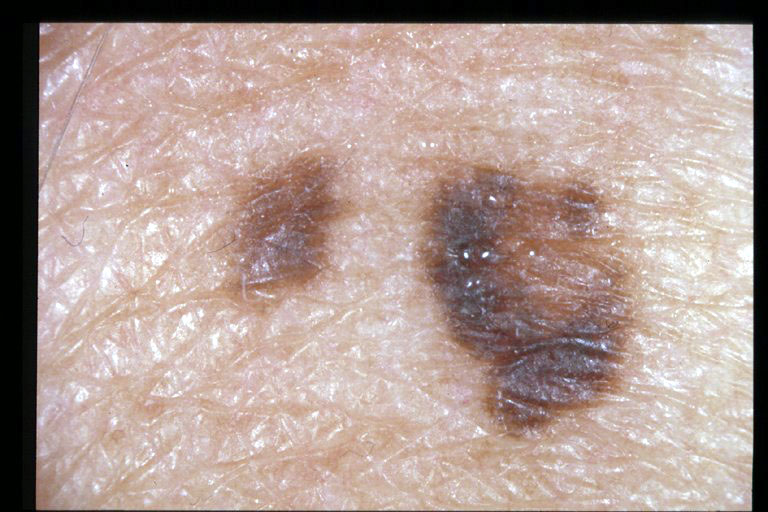
\includegraphics[width=\linewidth]{images/skin lesion/NEV/Aal005.jpg}
        \caption{Clinical image}
        \label{fig:nev_A}
    \end{subfigure}
    \begin{subfigure}[b]{0.48\linewidth}        %% or \columnwidth
        \centering
        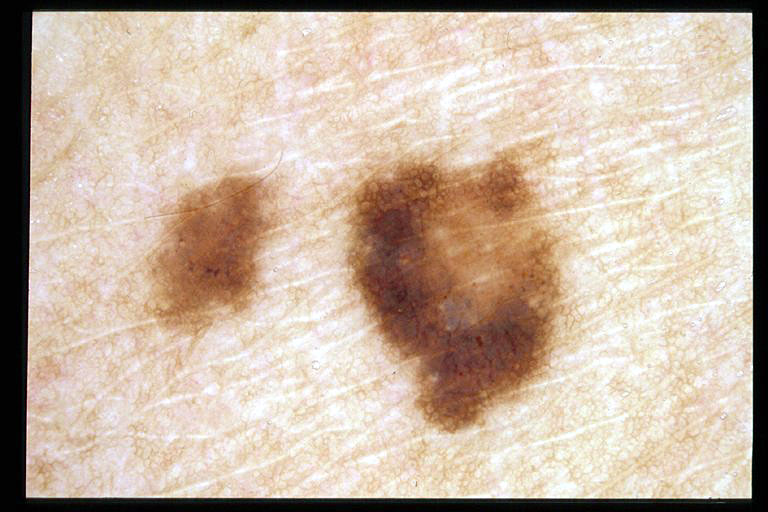
\includegraphics[width=\linewidth]{images/skin lesion/NEV/Aal006.jpg}
        
        \caption{Dermatoscopy  image}
        \label{fig:nev_B}
    \end{subfigure}
    \caption*{Source: https://derm.cs.sfu.ca/Welcome.html}
    \caption{Clark nevus with typical pigment network(7-point score: 0), absent streaks (score: 0), diffuse irregular pigmentation(score: 1), blue areas regression structures(score : 1), regular dots and globules (score : 0), absent blue whitish veil (score : 0), absent vascular structures(score : 0). Seven-point total score: 2}

    \label{fig:NEV_images}
\end{figure}
Cancerous (malignant) moles vary greatly in appearance. Some may show all of the changes listed above, while others may have only one or two unusual characteristics\cite{melanoma1}. \\ \\
\label{7ptRule}
The \textbf{Seven Point Checklist} was established by Argenziano et al.~\cite{Derm7ptData} for the dermoscopic differentiation between benign melanocytic lesions and melanoma. 
The dermoscopic evaluation,the 7-Point Check List, proceeds by calculating a score according to a scoring system, in which each tally is  assigned by evaluating irregular and atypical pattern, as shown in Table~\ref{table:1}.\\
A score equal to or greater than 3 predisposes to the diagnosis of melanoma (for practical example of the scoring system see Figures \ref{fig:MEL_images} and \ref{fig:NEV_images}).\\
This criteria is a widely used diagnostic method in the diagnosis of melanoma. Cutaneous malignancies can be identified with some certainty through this analytical procedure. All recognized melanomas have at least one of the seven main criteria defined by this system.
Numerous studies have confirmed the sensitivity of this method in the diagnosis of melanoma such as in \cite{7ptGeneralPractice}.
Its practicality consists in providing a public awareness of the visible characteristics of the tumor and thus shortening the waiting times for a specialized medical consultation and to ensure timely and appropriate intervention by the general doctor.


\begin{table}[]
\begin{tabular}{ |p{12cm}|p{0.8cm}|}
 \hline
 \multicolumn{2}{|c|}{\textbf{7-Point Score criteria}} \\
 \hline
 Dermoscopic pattern & Score \\
 \hline
 \textbf{Atypical network:} Combination of at least two types of pigment network (in terms of colour and thickness of the lines) asymmetrically distributed within the lesion & +2\\
 \textbf{Blue-white veil:} Irregular, structureless area of confluent blue pigmentation with an overlying white ‘ground-glass’ film. The pigmentation cannot occupy the entire lesion and usually corresponds to a clinically elevated part of the lesion & +2\\
 \textbf{Atypical vascular pattern:} Linear-irregular vessels, dotted vessels and/or milky-red areas not clearly seen within regression structures & +2 \\
\textbf{Irregular dots/globules:} More than three round to oval structures, brown or black in colour, asymmetrically distributed within the lesion & +1 \\
\textbf{Irregular streaks:} More than three brown to black, bulbous or finger-like projections asymmetrically distributed at the edge of the lesion and not clearly arising from network structures & +1 \\
\textbf{Irregular blotches:} Black, brown and ⁄or grey structureless areas asymmetrically distributed within the lesion & +1 \\
\textbf{Regression structures:} White scar-like depigmentation and/or blue pepper-like granules usually corresponding to a clinically flat part of the lesion & +1 \\
\hline
\end{tabular}
\caption{Dermoscopic criteria and scoring system of the classic version of the ‘seven-point checklist’ dermoscopic algorithm}
\label{table:1}
\end{table}
\clearpage
\section{Technical background}
\textbf{Deep neural networks}(DNN) mimic the human mind by replicating millions of connections between neurons, and basically consist of multiple layers interconnected through single units, the neurons. Depending on the inputs received, a neuron can be activated or not, producing a signal that is sent to another neuron on a hidden layer. This process continues until the signal has propagated to the output layer.
\subsection{Neurons}
Neurons are the building blocks of neural networks.
\begin{figure}[b]
    \centering
        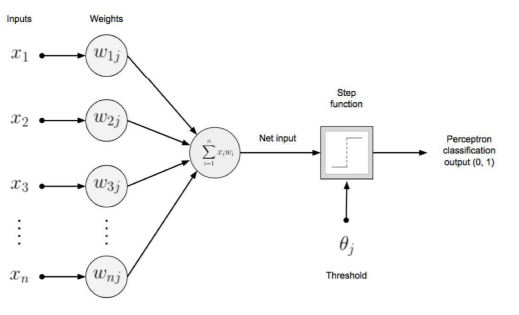
\includegraphics[width=0.7\linewidth]{images/deepLearning/neural block.png}
    \caption{Neuron structure \cite{DeepLearningApproach} }
    \label{fig:Neuron}
\end{figure}\\
Figure \ref{fig:Neuron} shows one of the basic structures of a neuron. A set of inputs are weighed and summed. The result is then used as an input for an activation function that determines how much the neuron will be activated by the signal received as an input. In the image:
\begin{enumerate}
    \item $x_i$ is the i-th input value.
    \item $w_i$ is the weight applied to $x_i$.
    \item $\theta$ is the activation threshold.
\end{enumerate}
The activation function is just a rule to determine how much will be activated; there are different types of activation functions, among which, the most common are the Sigmoid Function and the Relu Activation Function.\\
Sigmoid activation function produces an output in the range [0,1] while the ReLu produces $max(0,x)$ as output.
\subsection{Networks}
A neural network is made up of many neurons organized in layers. The figure shows a simple example of a neural network.
\begin{figure}[ht]
    \centering
        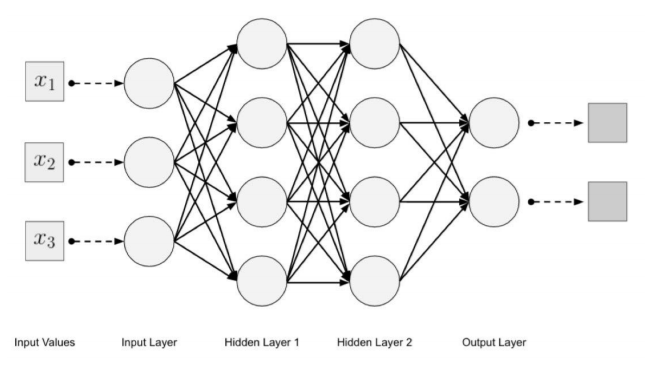
\includegraphics[width=0.7\linewidth]{images/deepLearning/network.png}
    \caption{Neural Network structure \cite{DeepLearningApproach} }
    \label{fig:Network}
\end{figure}
These types of networks use fully-connected layers which forward their outputs to all neurons in the next layer.
Each internal layer is called hidden layer. The output layer produces a set of relative probability values, related to a class. Typically, the final layer is a softmax, which converts the output of the previous one into a probability distribution.
\\ \\
The most common way to train a DNN is by supervising the training. Supervised learning is performed by using a set of input paired with the corresponding label output.
The network tries to mimic the training set, by modifying the network parameters during each training epoch, in order to reduce the value of a function, called cost function, which expresses the difference between the current output and the ground truth.
\\\\
The main common characteristic of deep learning methods is their focus on feature learning: automatically learning representations of data. Discovering features and performing a task is merged into one problem, and therefore both improve during the same training process \cite{deepLearningMRIimaging}.
Recently, deep learning has become one of the most successful techniques and achieved impressive performance in the computer vision field.
\textbf{Image classification} is the task of assigning an input image one label from a fixed set of categories. This is one of the core problems in Computer Vision that, despite its simplicity, has a large variety of practical applications.
The interest in deep learning made possible to apply classification techniques also in the medical field.

\subsection{Convolutional Neural Network}
\begin{figure}[]
    \centering
        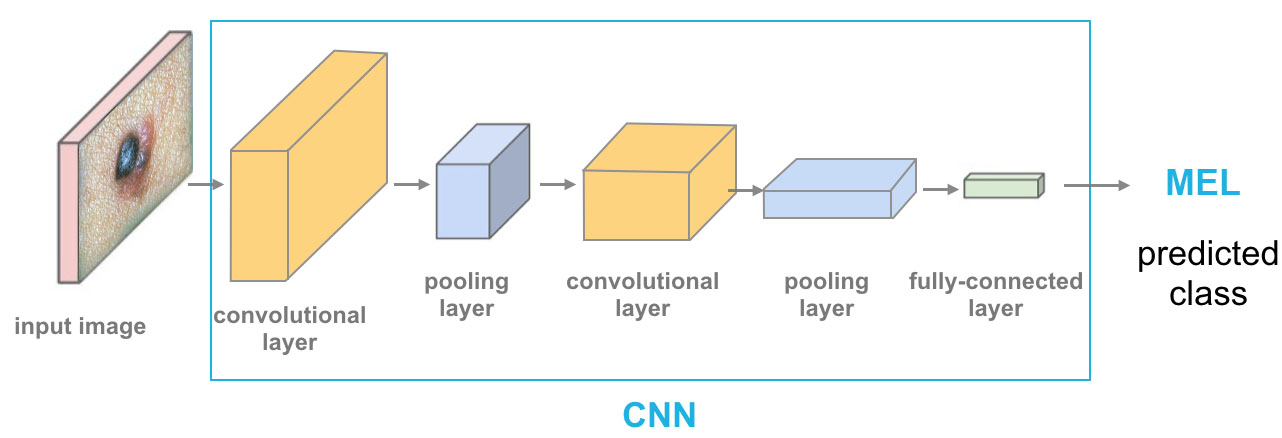
\includegraphics[width=0.9\linewidth]{images/CNN_ex.jpg}
    \caption{High level overview of CNN structures}
    \label{fig:CNN}
\end{figure}
\begin{figure}[hb]
    \centering
        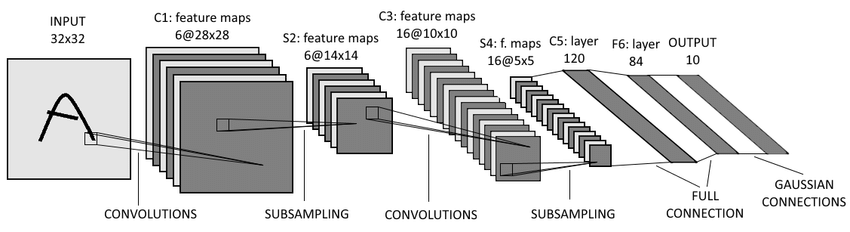
\includegraphics[width=0.7\linewidth]{images/deepLearning/leNet.png}
    \caption{LeNet-5 architecture \cite{LeNet} }
    
    \label{fig:LeNet}
\end{figure}
Image Classification is mostly achieved by using \textbf{Convolutional neural networks} (CNNs), a powerful way to learn useful representations of images and other un-structured data.\\
The name “convolutional neural network” indicates that the network employs a mathematical operation called convolution. Convolution is a specialized kind of linear operation. Convolutional networks are simply neural networks that use convolution in place of general matrix multiplication in at least one of their layers\cite{goodfellow}. A common example of a CNN architecture for image classification is shown in Figure~\ref{fig:CNN}. CNNs are a supervised learning method that learn the relationship between the input objects and the class labels and comprise two components: the hidden layers in which the features are extracted and, at the end of the processing, the fully connected layers that are used for the actual classification task. \\
In the context of image classification, a CNN in general does not process the input as a single block but as a composition of features. Unlike a common DNN, a CNN uses Fully-Connected layers only in the final part to produce the output, the classification probability distribution. 
\subsubsection{Architecture}
Figure~\ref{fig:CNN} shows an high-level structure of a CNN. Apart from the input layer, the middle layers achieve feature extraction while the final fully connected part performs classification.
Generally, feature extraction is performed by a repeated pattern. A convolutional layer is applied to the input,and then an activation function
and finally a Pooling layer, which reduces the information size.
An example of one of the first CNN created is shown in figure \ref{fig:LeNet}.
Unlike fully connected layers, convolution layers perform a convolution. The weights in a convolutional network are grouped into arrays called kernels.
Although they have a smaller width and height than the entrance, in basic CNN architectures they must match the depth.
Consider the input layer, an image usually has 3 dimensions: width, height and depth (in addition RGB encoding). So the first set of kernels must have a depth of three.\\
\begin{figure}[]
    \centering
        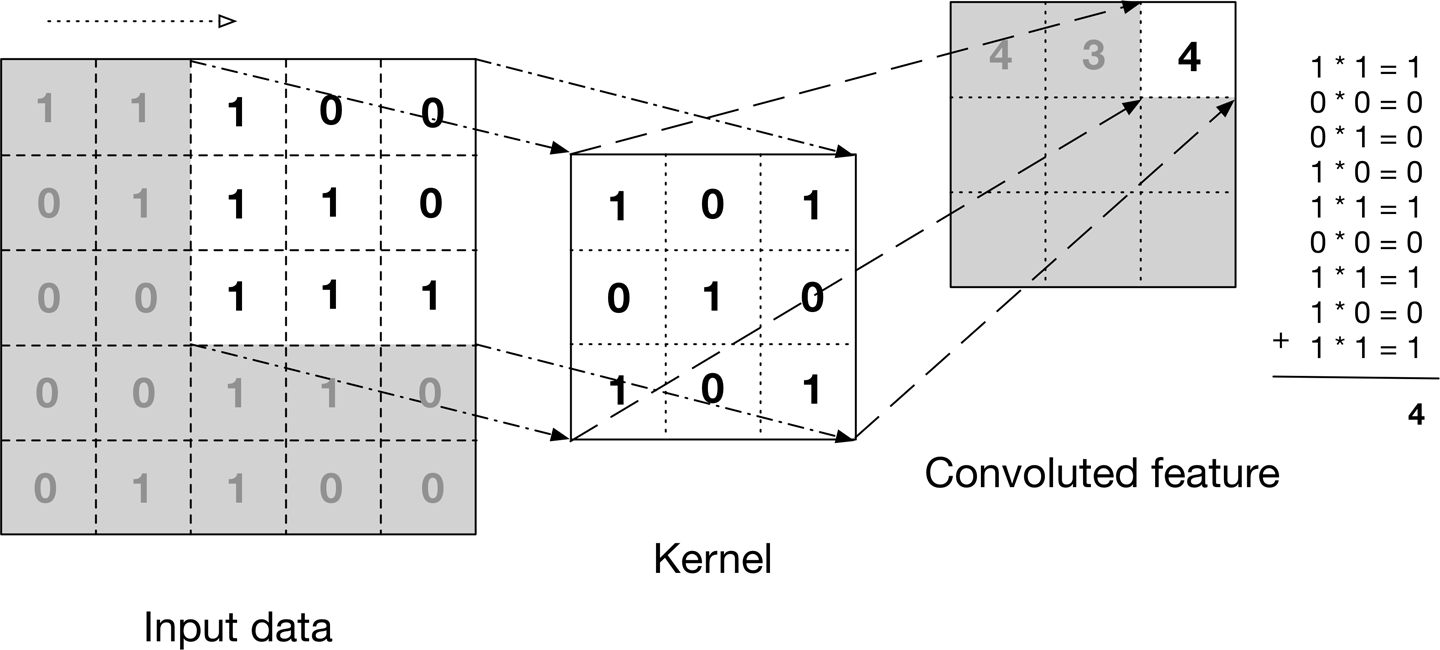
\includegraphics[width=0.7\linewidth]{images/deepLearning/conv.png}
    \caption{Convolution \cite{DeepLearningApproach} }
    \label{fig:Convolution }
\end{figure}
As shown in figure \ref{fig:Convolution  }, the convolution operation is applied by multiplying a kernel by an area in the input image. The result is then stored in the output matrix called feautere map. Once the input has been processed, the network uses the following kernel.\\
The \textbf{Pooling layer} combines similar features found in the feature map and helps prevent overfitting. The most common layer is Max Pooling, which extracts the maximum value.
Figure~\ref{fig:MaxPool } shows an example of Max Pooling with a stride of two.\\
\begin{figure}[]
    \centering
        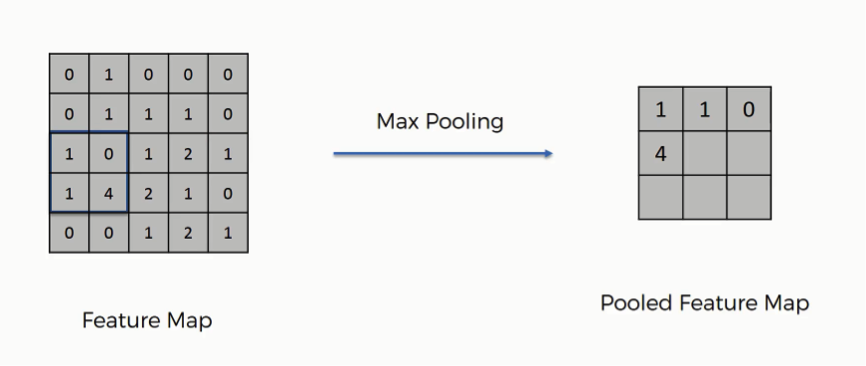
\includegraphics[width=0.7\linewidth]{images/deepLearning/maxpool.png}

    \caption{Max Pooling \cite{MaxPoolImage} }
    \label{fig:MaxPool }
\end{figure}
The \textbf{fully connected} layer takes the convolution or pooling output, flattens it and predicts the label that is most suitable for the input.
\subsection{Multi-task learning}
Recent works demonstrated that neural network also perform well in \textbf{multi-task learning}(MTL), that is the field, which takes care of learning more than one task at a time.
This approach showed that what is learned for each task can help other tasks be learned better.
In \cite{MTL}, performance of single task learning(STL) and MTL were compared; the related work showed that the extra information given in the MTL allowed to obtain better result than STL, especially in a real domain with medical background.\\
Sebastian Ruder in \cite{MTLoverview} presented two main MTL methods, shown in Figure~\ref{fig:MTLparadigms}, for Deep Learning: 
\begin{enumerate}[label=\Alph*]
\item Hard parameter sharing: this approach consists in sharing the hidden layers between all tasks, while keeping several task-specific output layers.
\item Soft parameter sharing: in this approach each task has its own model with its own parameters.
\end{enumerate}
Depending on the proposed strategy, a constraint is introduced among the parameters of the model.


\begin{figure}
    \centering
    \begin{subfigure}[b]{0.42\linewidth}        %% or \columnwidth
        \centering
        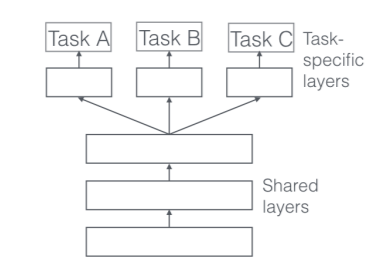
\includegraphics[width=\linewidth]{images/mtl hard.png}
        \caption{Hard parameter sharing approach}
        \label{fig:Hard}
    \end{subfigure}
    \begin{subfigure}[b]{0.54\linewidth}        %% or \columnwidth
        \centering
        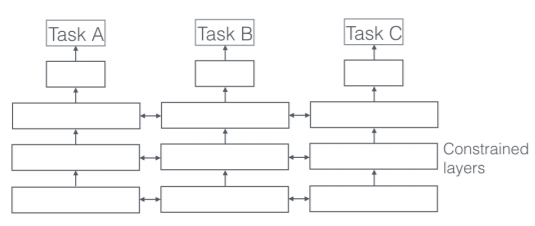
\includegraphics[width=\linewidth]{images/mtl soft.png}
        
        \caption{Soft parameter sharing approach}
        \label{fig:Soft}
    \end{subfigure}
    \caption{MTL sharing paradigms \cite{MTLoverview}}

    \label{fig:MTLparadigms}
\end{figure}

As shown in \cite{MTLoverview}, MTL performs well and it improves the learning process; it shows the following properties:
\begin{enumerate}
\item Implicit data augmentation: learning multiple tasks at the same time, permits to average the noise and provide a good representation for all the tasks.
\item Attention focusing: Sometimes differentiating relevant and irrelevant features for learning a task could be difficult due to noisy or limited data; MTL can help the model focus its attention on those features that actually matter as other tasks will provide additional evidence for the relevance or irrelevance of those features
\item Eavesdropping: learning some features for one task A could be more difficult than for a task B; learning them together allows task B to learn these features through B.
\item Representation bias: the representation of data will be generalized to provide a general structure to perform well with multiple tasks.
\item Regularization: by introducing an inductive bias, MTL reduces the risk of overfitting.
\end{enumerate}



\section{ML applications to skin lesion diagnosis}
Skin cancer detection and classification is a hot research topic since 1990's, and in literature many works were proposed \cite{7ptCNNforMel,estevaMLinDerm,mtl7ptCoppola,Kawahara,MLinDermat,HanWork}
Machine learning algorithms have the potential to improve the dermatologist’s practice from diagnosis to personalized treatment \cite{MLinDermat}. 
Supervised learning is the most common type of learning used in dermatology \cite{MLinDermat}.
A significant research regarding skin lesion classification is represented by the work of Esteva et al.~\cite{estevaMLinDerm}, that collected 129450 macroscopic images consisting of 2032 diseases. A Deep Neural Network (DNN) was trained on an Inception-V3 architecture using transfer learning, with weights pre-trained on ImageNet~\cite{ImageNet}. The prediction performances were tested against dermatologists on biopsy-proven clinical images.
Han et al.~\cite{HanWork} have merged different public datasets with a proprietary dataset to gather over 20.000 samples of macroscopic images, with 12 classified diseases. The ResNet \cite{Resnet} network architecture with weights pre-trained on ImageNet was used for this approach. Transfer learning was performed by freezing the weights of lower-level layers, in order to preserve the basic feature extraction from images.
The interest in skin lesion diagnosis using dermoscopic images increased after the ISIC dataset challenge was introduced \cite{IsicChallenge}, alongside with the benchmark for evaluation. The best performing approach was obtained by using an ensemble of DNNs and enhancing the number of samples by merging other datasets\cite{multiDataset}. \\
There are also methods developed upon both types of images and including additional metadata, working on the derm7pt dataset \cite{Kawahara}, which includes information for the 7 attributes used in the 7-point checklist diagnosis method.
Kawahara et al.\cite{Kawahara} developed a model for diagnosis prediction by joining two InceptionV3 networks with pre-trained weights on ImageNet \cite{ImageNet}. Since the 7-point checklist and the diagnosis are related tasks, the results are improved due to the higher generalization of a multi-task model. Furthermore, the model performance is increased by combining the outputs of the complementary modalities. During training all the modalities are available, whereas for the inference stage one or a specific combination of modalities can be used.
In Coppola et al.~\cite{mtl7ptCoppola} a MTL application was proposed. The authors of this work implemented a MTL method that learns what to share between tasks through gates, which allows the inspection of the relationships learned by the network. By means of gate blocks they allow tasks to share useful features. \\ 
Alzahrani et al.~\cite{7ptCNNforMel} developed a method for skin lesion detection and melanoma diagnosis from dermoscopy images by combining seven-points checklist criteria with convolutional neural networks. The proposed models have been realised by incorporating automated lesion feature extraction achieved by multi-input CNN considering standardised images (dermoscopy) and non-standardised images (clinical). This methos is similar to a concept bottleneck model, in which it first predicts the 7-point checklist attributes, and then use them for melanoma diagnosis, by applying 7-point algorithm.

 


\graphicspath{{chapters/chapter3/}}
\chapter{Dataset} \label{chapter4}
Experiments have been carried out on the Derm7pt dataset (collecting images from the {Interactive Atlas of Dermoscopy}~\cite{Derm7ptData} ), which was publicly released with \cite{Kawahara}.The dataset consists of 1011 cases of skin lesion, previously annotated by doctors. For each case, data are available in different modalities(e.g. metadata, clinical and dermatoscopic images), however this work only considers dermatoscopic images, which provide better resolution and allow to appreciate better the patterns on the lesion that are necessary for the 7-point criteria.
\begin{table}[]
\centering
\begin{tabular}{|l|r|r|}
\hline
\multicolumn{3}{|c|}{\textbf{Derm 7pt}} \\ \hline
 & \multicolumn{1}{l|}{\textit{NEV}} & \multicolumn{1}{l|}{\textit{MEL}} \\ \hline
Training set & 256 & 90 \\ \hline
Validation set & 100 & 61 \\ \hline
Test set & 219 & 101 \\ \hline
\textit{Total} & 575 & 252 \\ \hline
\end{tabular}
\caption{Number of cases in the dataset, stratified by split. The dataset consists of only Nevus and Melanoma cases; training, test and validation subsets were split following the work of Kawahara et al.\cite{Kawahara} }
\label{table:dataset}
\end{table}

The dataset was split in training, test and validation subsets as in the work by Kawahara et al. \cite{Kawahara}. However this work only considers the Nevus and Melanoma cases; thus, the samples belonging to other types of of lesions have been discarded. The remaining number of samples is 827, split according to the details in Table ~\ref{table:dataset}.\\
The final datasets were unbalanced due to the minority of melanoma cases.
Possible solutions have been studied to compensate for the imbalance were oversampling and undersampling of the dataset; in \cite{mtl7ptCoppola,Kawahara} a method to balance the data for each batch were proposed. In this work an oversampling technique was employed by duplicating melanoma cases in the training set, and by finally applying data augmentation\footnote{Data augmentation: technique to increase the diversity of the training set by applying random (but realistic) transformations such as image rotation. The proposed work deploys horinzontal and vertical flip, and crop, on the training images.}.
This solution solves only the problem of the imbalance on the DIAG task and not on the remaining 7 tasks, for which no technique has been enforced.
For each case 8 labels are available as summarized in Table~\ref{table:3} and they represent the 8 tasks to learn by the architectures implemented in this work.




\begin{table}[]
\begin{tabular}{ |p{6.2cm}|p{4.5cm}||p{1.6cm}|}
 \hline
 Task name & Classes & 7pt-Score \\
 \hline
 \textbf{Diagnosis (DIAG)} & NEV, MEL & \\\hline
 \textbf{Pigment network (PN)} & ABS(0), TYP(0), ATP(2) & +2\\\hline
 \textbf{Blue Whitish Veil (BWV)} & ABS(0), PRS(2) & +2\\\hline
 \textbf{Vascular Structure (VS)} & ABS(0), REG(0), IR(2) & +2 \\\hline
\textbf{Dots and Globules (DaG)} & ABS(0),  REG(0), IR(1) & +1 \\\hline
\textbf{Streaks (STR)} & ABS(0),  REG(0), IR(1) & +1 \\\hline
\textbf{Pigmentation (PIG)} & ABS(0),  REG(0), IR(1) & +1 \\\hline
\textbf{Regression structures (RS)} & ABS(0),  REG(0), IR(1) & +1 \\
\hline
\end{tabular}
\caption{The first task (DIAG) indicates the final diagnosis of the lesion, whereas the following are the 7 attributes that are used
in the 7-point checklist.NEV:nevus; MEL: melanoma; ABS: absent; TYP: typical; ATP: atypical; PRS: present; REG: regular; IR: irregular.}
\label{table:3}
\end{table}


\graphicspath{{chapters/chapter4/}}
\chapter{Methods} \label{chapter3}

This section summarizes the theory behind the techniques implemented in the experiments.  The first paragraph concerns Logistic Regression, a classic supervised machine learning method for classification. Then follows a section with a brief description of the implemented deep learning architectures.  Finally, the general framework of CBM is presented.
\section{Logistic Regression}
\textbf{Logistic Regression(LR)} is a supervised learning classification algorithm used to predict the probability of an input to belong to a target class. The nature of target or dependent variable is dichotomous, which means that the probability of the output to belong to a class will be $P$, while $(1-P)$ if it belongs to the other class(where $P$ is a number between 0 and 1).\\ 
Logistic Regression is achieved by applying Sigmoid function on linear regression:
\begin{equation}
p = \frac{1}{1 + e^{-(\beta_0 + \beta_1 x_1 + \beta_2 x_2 + ... +\beta_n x_n)}    }
\label{LReq}
\end{equation}
The Linear Regression Function is defined as:
\begin{equation}
y = \beta_0 + \beta_1 x_1 + \beta_2 x_2 + ... +\beta_n x_n
\end{equation}
where, $y$ is dependent variable and $x_1, x_2 ...$ and $x_n$ are explanatory input variables, the Sigmoid Function is defined as: 
\begin{equation}
p = \frac{1}{1+e^{-y}}
\end{equation}
The sigmoid Function gives an ‘S’ shaped curve that can take any real-valued number and map it into a value between 0 and 1.
\section{Deep learning architectures}
In the literature, models that perform well in image classification tasks and give good results also in the medical field have been proposed. Complex architectures already pre-trained on large dataset, have been made available in many frameworks, such as Tensorflow\cite{tensorflow2015-whitepaper}.
The following paragraphs describe the structures of the 2 networks used in the experiments, InceptionV3 and ResNet101v2, by using transfer learning.
\subsection{InceptionNet}
\begin{figure}[b]
    \centering
    \begin{subfigure}[b]{0.48\linewidth}        %% or \columnwidth
        \centering
        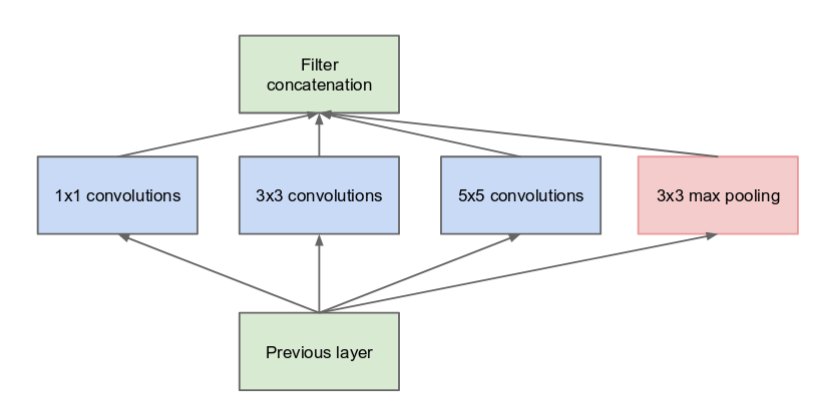
\includegraphics[width=\linewidth]{images/incNet/incnaivemodule.png}
        \caption{Inception Module, naive version}
        \label{fig:incNaiveMod}
    \end{subfigure}
    \begin{subfigure}[b]{0.48\linewidth}        %% or \columnwidth
        \centering
        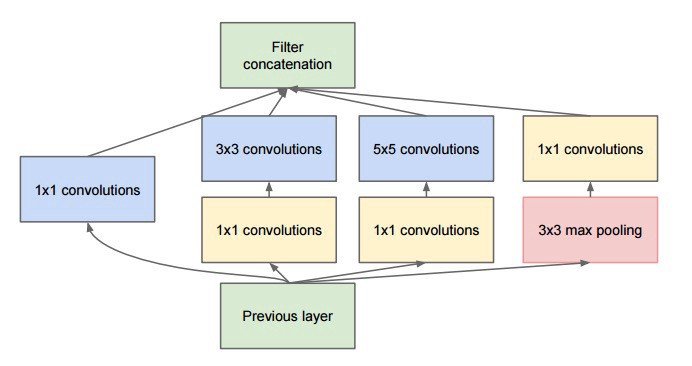
\includegraphics[width=\linewidth]{images/incNet/incmodule.jpeg}
        
        \caption{Inception Module with dimension reductions}
        \label{fig:incModule}
    \end{subfigure}
    \caption{Inception Module}

    \label{fig:NEV_images}
\end{figure}

\begin{figure}[ht]
    \centering
        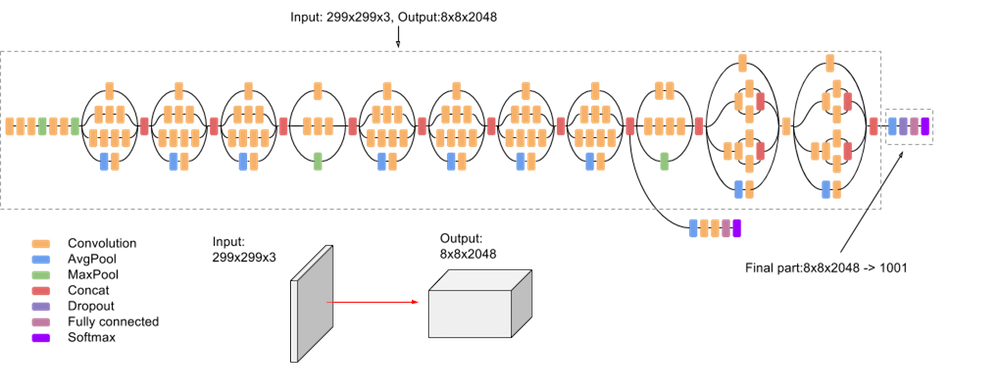
\includegraphics[width=\linewidth]{images/inception_v3_architecture.png}
    \caption{InceptionV3 architecture}
    \label{fig:IncV3}
\end{figure}
\textbf{InceptionV3(IncNet)} is a widely-used image recognition model that has been shown to attain greater than 78.1\% accuracy on the ImageNet dataset~\cite{ImageNet}. The model is the result of many works developed by multiple researchers over the years \cite{IncNet}.\\\\
Inception nets are characterized by a reduced depth at the expense of width; this property allows to have a lower computational complexity than deep networks. \\
This kind of networks are made up of modules called \textbf{Inception Modules}, which allow to have filters with multiple sizes on the same level. The figure~\ref{fig:incNaiveMod} shows the "naive" inception module: it performs convolution on an input with 3 different filters (1x1, 3x3, 5x5). Additionally, max pooling is performed. The outputs are concatenated and sent to the next layer.
Due to the computational effort, extra 1x1 convolutions have been added to these modules, figure~\ref{fig:incModule}.\\
Furthermore, smart factorization methods have been implemented, to factor bigger convolutions(7x7, 5x5) into more convolutions of reduced sizes; they factor the convolutions of the nxn filter size into a combination of 1xn and nx1 convolutions.\\
Other important properties of the network are:
\begin{enumerate}
    \item RMSProp Optimizer.
\item Factorized 7x7 convolutions.
\item BatchNorm in the Auxillary Classifiers.
\item Label Smoothing (A type of regularizing component added to the loss formula that prevents over fitting).
\end{enumerate}
The IncNet is formed by the Inception Modules, and auxiliary classifiers are added in the middle part of the network to apply softmax on the output and to compute an auxiliary loss.\\
The architecture for the InceptionV3 is showed in figure~\ref{fig:IncV3}; the model itself is made up of symmetric and asymmetric building blocks, including convolutions, average pooling, max pooling, concats, dropouts, and fully connected layers. Batchnorm is used extensively throughout the model and applied to activation inputs.
This architecture was trained using a dataset of 1,000 classes from the original ImageNet dataset which was trained with over 1 million training images, while the Tensorflow implementation has 1,001 classes which is due to an additional "background" class not used in the original ImageNet.

\subsection{ResNet}
\textbf{ResNet101V2(ResNet)} is a convolutional neural network that is 101 layers deep. ResNet101V2, as IncNet, was trained on ImageNet.\\
The ResNet architecture is built to address the vanishing gradient problem.
The vanishing gradient problem, argued and discussed in \cite{vanishinGradient}, is a phenomenon that creates difficulties in the training of deep neural networks through the back-propagation of the error through stochastic descent of the gradient. \\
So with ResNet, the gradients can flow directly through the skip connections backwards from later layers to initial filters, solving problem related to back-propagation; this is achieved by introducing a new neural network layer, the Residual Block, shown in figure~\ref{fig:ResBlock}. \\
\begin{figure}[]
    \centering
        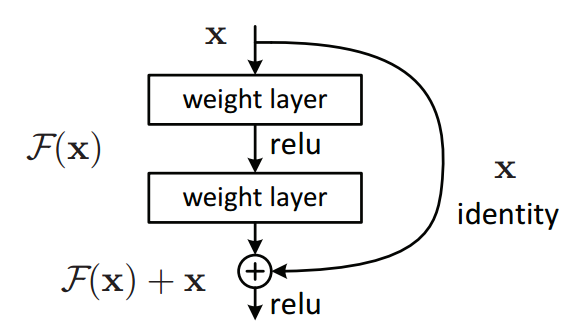
\includegraphics[width=0.7\linewidth]{images/resnet/residualblock.png}
    \caption{Residual Block}
    \label{fig:ResBlock}
\end{figure}
A ResNet is a very deep CNN, consisting of many layers, which with the aid of the technique of skip connection has opened the way to residual networks. Skip connection is the key to training a large number of levels, without losing performance.
Skip connection allows a fast compute of the cost function, by skipping to each residual block during the gradient backpropagation\cite{Resnet}.
\subsection{Transfer Learning}
\textbf{Transfer Learning:}
CNNs can either be trained from scratch where all its parameters are tuned for the problem, or they can be tuned towards the problem from an already pre-trained CNN. This method can be particularly useful for medical applications since it does not require as much training data, which can be hard to get in medical situations \cite{TransferLearningMedicalBackground}. 
A common way to use transfer learning is by loading a model(e.g. ResNet101, InceptionV3) with weights pre-trained on a large database of images annotated with labels (e.g. ImageNet\cite{ImageNet}) and by excluding the fully-connected layer at the top of the network. Generally a new classification layer is added, that is specific to the new task. The model weights are then fine-tuned on the task-specific dataset. In this way, the model should retain basic filters already learned by training on the previous data, resulting in better accuracy and quicker convergence.
\\
\section{Concept BottleNeck Models} \label{sectionCBM}
\textbf{Concept Bottleneck Models(CBM):} are models that first predict an intermediate set of human-specified concepts $c$, then use $c$ to predict the final output $y$\cite{CBM}.
Consider predicting a target $y\in\R$ from input $x\in\R^d$; Firstly, a CBM will predict a vector of $k$ concepts $c\in\R^k$. Then it will use the predicted concepts to estimate the target variable $y$\\
A CBM has the following form, $g(f(x))$, where $f:\R^d \longrightarrow \R^k$ maps an input $x$ into the concepts space and $g:\R^k \longrightarrow \R$ maps concepts into a final prediction. So a CBM will predict $\hat{y}=g(f(x))$ by predicting the concepts $\hat{c}=f(x)$ and $y=g(\hat{c})$. \\
Different ways to learn a concept bottleneck model were studied in \cite{CBM}, but this work only consider:
\begin{enumerate}
    \item The independent bottleneck, that learns ${g}$ and ${f}$ independently: $f$ is trained on the raw inputs and $g$ on the true concepts. But, at test time, ${g}$ takes the predicted concepts $\hat{c}={f}(x)$ 
    \item The sequential bottleneck, first learns ${f}$ in the same way as above. It then uses the concept predictions $\hat{c}$ to learn ${g}$.
\end{enumerate}

\section{Categorical Cross-Entropy Objective function}
\textbf{Categorical Cross-Entropy Loss:} is a Softmax activation plus a Cross-Entropy loss. By using this loss,a CNN will be train a CNN to predict a probability over the 
C classes for each image. It is used for multi-class classification.\\
Softmax function(\ref{softmax}) extends the idea of Sigmoid Function into a multi-class problem,by assigning decimal probabilities to each class. Below softmax function:
\begin{equation}
    softmax(x)_i = \frac{\exp(x_i)}{\sum_{j}^{ }\exp(x_j)}
    \label{softmax}
\end{equation}
where, $x_i$  is the propability for the i-th class and $x_j$ the propability for others classes.
Categorical Cross-entropy measure the difference between two probability distributions for a given random variable and calculates the loss of a class by computing the following sum:
\begin{equation}
    CCE = {\sum_{i}^{ }x_i \log(softmax(\hat{x}_i))}
    \label{softmax}
\end{equation}
where $\hat{x}_i$ is the i-th scalar value in the model output, $x_i$ is the corresponding target value.\\


\graphicspath{{chapters/chapter5/}}
\chapter{Results} \label{chapter5}
\label{exp_Results}
\section{Experiments}
% Please add the following required packages to your document preamble:
% \usepackage{multirow}
\begin{table}[]
\begin{tabular}{|l|l|l|l|l|}
\hline
 &
  Name &
  Base &
  \begin{tabular}[c]{@{}l@{}}Classification \\ Head(s)\end{tabular} &
  Loss Function \\ \hline
\multirow{4}{*}{\begin{tabular}[c]{@{}l@{}}Single Task \\ Learning (STL) \\ for diagnosis \\ prediction\end{tabular}} &
  \textit{IncNet} &
  IncNet &
  F.C. &
  Cross-Entropy \\
 & \textit{IncNet*+L.R.}               & IncNet* & L.R.     & L2 penalty     \\
 & \textit{ResNet}                     & ResNet  & F.C.     & Cross-Entropy \\
 & \textit{ResNet*+L.R.}               & ResNet* & L.R.     & L2 penalty     \\ \hline
\multirow{3}{*}{\begin{tabular}[c]{@{}l@{}}Muli Task Learning\\ (MTL) for Concepts \\ prediction\end{tabular}} &
  \textit{IncNet$_{MTL}$} &
  IncNet &
  F.C. x 7 &
  Cross-Entropy \\
 & \textit{IncNet*$_{MTL}$+L.R.}       & IncNet* & L.R. x 7 & L2 penalty     \\
 & \textit{ResNet*$_{MTL}$+L.R.}       & ResNet* & L.R. x 7 & L2 penalty     \\ \hline
\multirow{6}{*}{\begin{tabular}[c]{@{}l@{}}Concept Bottleneck \\ Models (CBM) \\ for diagnosis \\ prediction\end{tabular}} &
  \textit{Ind | IncNet$_{MTL}$} &
  IncNet &
  L.R. &
  L2 penalty \\
 & \textit{Seq | IncNet$_{MTL}$}       & IncNet  & L.R.     & L2 penalty    \\
 & \textit{Ind | IncNet*$_{MTL}$+L.R.} & IncNet* & L.R.     & L2 penalty     \\
 & \textit{Seq | IncNet*$_{MTL}$+L.R.} & IncNet* & L.R.     & L2 penalty     \\
 & \textit{Ind | ResNet*$_{MTL}$+L.R.} & ResNet* & L.R.     & L2 penalty    \\
 & \textit{Seq | ResNet*$_{MTL}$+L.R.} & ResNet* & L.R.     & L2 penalty     \\ \hline
\end{tabular}
\caption*{*weights are frozen}
\caption{Representation of models used for experiments. F.C.: Fully Connected layer; L.R.: Logistic Regression.}
\label{table:modelsTable}
\end{table}
The goal of this work, is to develop a model able to detect Melanoma in dermoscopic images of skin lesions, by learning first a set of human-understandable concepts. \\
To do this, the Concept Bottleneck Framework (Sec. \ref{sectionCBM}) was employed, by designing models that first predict the clinical attributes from 7-poin checklist method(Sec. \ref{7ptRule}) and then use those for the final diagnosis of the lesion. \\
These models have then been compared with the more standard Single Task Learning approaches, which learn the diagnosis end-to-end without intermediate concepts.\\ 
All proposed models, shown in Table~\ref{table:modelsTable}, use an IncNet or a ResNet pretrained over ImageNet as base model. The class-specific layer of either models was replaced with a trainable layer related to the task. \\

\subsection{Single Task Learning for Diagnosis prediction}
Single Task Learning architectures are end-to-end models $g$ that from an input $x$ (Dermatoscopy image) predict directly the diagnosis, by extracting hidden features $h=f(x)$, and by using them to predict $\hat{y}_{DIAG}=g(f(x))$, by means of a classification head. Figure~\ref{fig:StLimage} shows a standard representation for a STL model.\\
The first two implementation are the \emph{IncNet} and the \emph{ResNet}, which use respectively as base $f$ an InceptionV3 and a ResNet101V2 imported from TensorFlow library \cite{tensorflow2015-whitepaper}.
In both networks, the final layer was replaced with a Fully Connected layer, the classification head $g$, specific to the Diagnosis task and categorical cross-entropy loss was used. Training has been done using a custom Keras Sequence with augmentation on training set, by flipping and cropping images, on 250 epochs with a patience of 50 epochs and a learning rate of
0.001 for ADAM optimizer(See Sec. \ref{IncNet}, \ref{ResNet} for more training details).\\
The experiments \emph{IncNet*+L.R.} and \emph{ResNet*+L.R.} were developed similarly to the method presented in the work of Kawahara et al.\cite{Kawahara}. By using respectively an InceptionV3 and a ResNet101V2 as base $f$ of the networks. The models were initialized with weights trained on the ImageNet dataset; keeping them frozen, they were employed to extract a set of features $h=f(x)$. Extracted features $h$ and related DIAG labels, were employed then, for the training of the Logistic Regression model $g$ added to the head of the network. The Logistic Regression models were implemented by using the scikit learn library \cite{scikit-learn}, in which a L2 penalty loss function is used. Logistic Regression model was trained using the extracted features.
\subsection{Multi Task Learning for Concepts prediction} \label{sectionMTL}
Multi task learning models have the form of $\{g_t(f(x)),\; \forall t \in \{ PN, BWV, \hdots \} \}$ where $f$ performs the extraction of hidden features from a base model and $g_t$ predicts the 7 tasks of the 7-point checklist rule, according to Table~\ref{table:3}. General architecture of MTL models is showed in Figure~\ref{fig:x_cimage}.\\ 
The first MTL model presented is the \emph{IncNet$_{MTL}$}, in which an InceptionV3 was joined to a block of Dense layer, followed by 7 Fully Connected layers, each of them related to one of the 7 tasks. For each block, Categorical Cross-Entropy loss function was implemented. The resulting model was trained on the training set over 200 epochs with a patience of 30, and a stochastic gradient descent (SGD) having a learning rate of 0.001 as optimization algorithm(See Sec. \ref{MtlIncNet} for more training details).\\
\emph{IncNet*$_{MTL}$+L.R.} and \emph{ResNet*$_{MTL}$+L.R.} models, use a frozen base model trained on ImageNet to extract features that are then used ad input to 7 different Logistic Regressions (one per task). Each  Logistic Regression model was trained using extracted features as input and each task's label as ground truth.
\subsection{Concept-Bottleneck Models for Diagnosis prediction}
Concept Bottleneck architectures have the form $\tilde{g}_{DIAG} \left( g_{PN} \left( f(x) \right),\;  g_{BWV} \left( f(x) \right),\; \hdots \right)$, where $f(x)$ performs the features extraction from a base model, $g_t$ the intermediate concept prediction for every attribute $t$ in the 7-point checklist (Sec. \ref{7ptSection}) and $\tilde{g}$ performs the prediction of the main classification task using the predicted concepts $\hat{c} = \{g_t(f(x)),\; \forall t \in \{ PN, BWV, \hdots \} \}$ represented in Table~\ref{table:3}, related to the 7pt checklist rule. Independent and sequential architecture were implemented by joining the models for concepts predictions to a Logistic Regression classifier. \\
In the Independent models the functions to predict the concepts are trained Independently from the one to predict the main task. Three different approaches to predict the tasks have been described in the previous section(Sec. \ref{sectionMTL}). The function to predict the diagnosis is trained using the ground truth for the concepts as input.
Conversely, in the Sequential model the two models are trained one after the other. First the concepts predictor is trained to generate the prediction $\hat{c}$. Then the logistic regression to predict the diagnosis is trained on the predicted concepts $\hat{c}$.\\
General architecture of CBM is showed in Figure \ref{fig:CBMimage}, where as $g(f(x))$ it takes one of the proposed models for concepts prediction, and as $\tilde{g}(\cdot)$ a Logistic Regression model.
\begin{figure}[]
\centering
  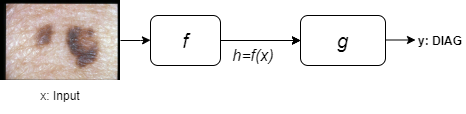
\includegraphics[width=.7\linewidth]{images/model/STL.png}
  \caption{Architecture for end-to-end models that go directly from raw input $x$ to final target $y$.}
  \label{fig:StLimage}
\end{figure}


\begin{figure}[]
\centering
  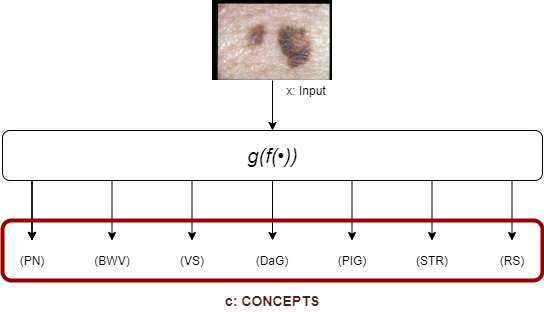
\includegraphics[width=.7\linewidth]{images/model/MTL (2).png}
  \caption{Architecture for MTL models}
  \label{fig:x_cimage}
\end{figure}

\begin{figure}[]
\centering
  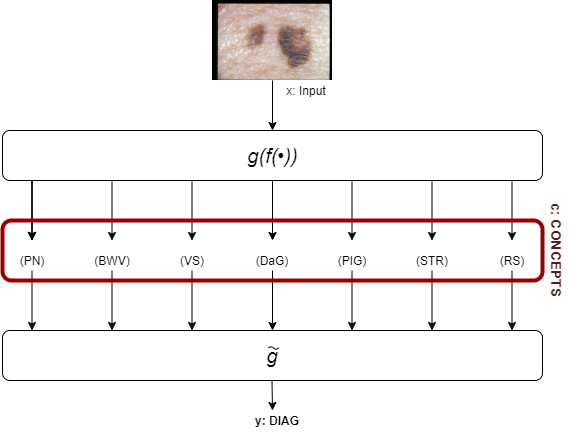
\includegraphics[width=.7\linewidth]{images/model/CBm (1).png}
  \caption{General architecture for Concept Bottleneck models}
  \label{fig:CBMimage}
\end{figure}
\subsection{7-point Checklist Rule}
7-point Checklist Rule is applied using the ground truth concepts from the test set, and it diagnoses Melanoma if a score greater than or equal to 3 was obtained.

\section{Results}
The performance of all proposed methods for lesion identification and melanoma diagnosis was evaluated using accuracy, recall, F1 score on MEL label and precision, which can be defined as follows:
\begin{equation}
    Accuracy = \frac{tp + tn}{tp + tn + fp +fn}
\end{equation}
\begin{equation}
    Recall = \frac{tp}{tp +fn}
\end{equation}
\begin{equation}
    Precision = \frac{tp}{tp + fp}
\end{equation}
\begin{equation}
    F1 score =2 \cdot \frac{precision \cdot recall}{precision + recall}
\end{equation}
where $tp$,$tn$,$fp$ and $fn$ refer to true positive, true negative, false positive, and false negative, respectively. The baseline results obtained from proposed system for melanoma diagnosis are presented in Table~\ref{table:results}, and accuracy on concepts predictions, is shown in Table~\ref{table:ConceptsAccuracy}.
The performance of the models were measured by performing stratified 5-fold cross-validation on the test set. The test set was divided into 5 folds, balanced according to the true label of diagnosis.\\ \\
In Single task learning prediction, the best performance was achieved by \emph{ResNet} model trained using Transfer Learning, which obtained about $81.25\pm3.28\%$ in Accuracy metric. Comparable performance were obtained by \emph{ResNet*+L.R.}, even if it wasn't trained on Derm7pt images; this model shows better performance even than \emph{IncNet}. Hierarchies implementing ResNet101v2 showed the best metrics in single task learning, and fine-tuned models remained the most performing. However satisfactory results were also obtained by simply freezing the weights in \emph{IncNet*} and \emph{ResNet*} where, the feature extractors were learned for general images in ImageNet. \\\\
Also for the MTL models we find that the fine-tuned models performed better than models in which the weights were frozen. Table~\ref{table:ConceptsAccuracy} summarizes the performance of models in predicting the concepts alone. \emph{IncNet$_{MTL}$} trained on Derm7pt, reports the best accuracy in concepts predictions, with an average value of $66.97 \pm5.84\%$, compared to $65.93\pm5.03\%$ and $65.93\pm4.84  \%$ obtained with \emph{IncNet*$_{MTL}$+L.R.} and \emph{ResNet*$_{MTL}$+L.R.} models.\\\\
The best bottleneck model were the \textit{Seq | IncNet$_{MTL}$} and \textit{Seq | ResNet$_{MTL}$} that achieved $77.50\pm8.07\%$ and $76.56\pm3.13\%$ accuracy respectively on Diagnosis prediction.\\
In each CBM implementations, Sequential bottleneck models, seem to be more accurate than Independent models, also if the sequential $f$ model is trained on predicted concepts, while independent $f$ model is trained on the true concepts.
\\\\
The model that accomplish the best performance was the one with the "black-box" nature, the \emph{ResNet} model. STL learning therefore remains the finest, but it can't provide an explanation of how it predicts the final target $y$, unlike CBM that provides a set of human-understandable specified concepts for a clear explanation.
\\\\
The clinical rule used by dermatologists still seems to be the most effective. In fact, by applying the ground truth score of each concepts taken from the test set, it obtains the best accuracy compared to the proposed architectures. In particular, it showed the best results for the F1 score metric related to the MEL label, obtaining $ 78.43\pm4.77 \% $ far higher than the scores achieved by the proposed models.\\
For more details on model predictions see section \ref{chapter7}, which shows the related confusion matrices for each architecture.
\\\\
Overall, the architectures developed perform adequately and they stand up to other works proposed in the literature.
Comparing with other approaches that used the same dataset is challenging as often different subsets of the data are used and especially, because this work only considers melanoma and nevus cases of the Derm7pt dataset.
In \cite{Kawahara,mtl7ptCoppola} the DIAG task and the 7 tasks were put on the same level without taking into consideration any possible intermediate implementation;
Kawahara et al.~\cite{Kawahara} achieved an accuracy\footnote{Kawahara et al.\cite{Kawahara} results refer to experiment \textit{x-combine}, which uses additional data during training} of $74.2\%$ but taking into consideration all the labels of the DIAG task (BCC, NEV, MEL, MISC, SK) and not only MEL and NEV labels; while they achieved an average value of $73.6\%$ on concepts prediction.
Coppola et al.~\cite{mtl7ptCoppola} achieved an accuracy\footnote{Coppola et al.\cite{mtl7ptCoppola} results refer to experiment \textit{binary}, which considers only 2 output classes for DIAG task} of $77.2\%$ and an average value of $61.3\%$ on the 7 attributes prediction.\\
The \textit{Seq | IncNet$_{MTL}$} implementation performed better than the 2 results achieved in \cite{Kawahara,mtl7ptCoppola}, providing a better explanation of how the diagnosis was computed, although it must be remembered that it only distinguishes between NEV and MEL labels.


\begin{table}[]
\begin{tabular}{|l|c|c|c|c|}
\hline
\textbf{Model}  & \multicolumn{1}{c|}{Accuracy}      & \multicolumn{1}{c|}{Recall}  & \multicolumn{1}{c|}{F1 Score} & \multicolumn{1}{c|}{Precision}\\ \hline
\emph{IncNet}   & $78.43 \pm 2.50$    & $74.36\pm12.17$     &  $64.82\pm4.75$   & $75.13 \pm 9.02$\\
\emph{ResNet}    & \boldsymbol{$81.25 \pm 3.28$}   & $76.69\pm 14.68$ &    \boldsymbol{$67.96 \pm 7.15$}& \boldsymbol{$78.68 \pm 6.98$}\\
\emph{IncNet*+L.R.}   & $74.06\pm6.60$    & $71.17\pm10.96$ & $60.75\pm9.74$& $70.37\pm 6.98$             \\ 
\emph{ResNet*+L.R.}   & $80.31\pm2.89$      & \boldsymbol{$76.77\pm 12.80$} & $67.79\pm7.02$ & $77.37\pm14.29$          \\ 

\hline
\textit{Ind | IncNet$_{MTL}$} & $77.50 \pm8.36$ & $74.45\pm13.62$ & $65.12\pm12.50$ & $74.42\pm14.27$\\ 
\textit{Seq | IncNet$_{MTL}$} & \boldsymbol{$77.50 \pm 8.07$}& \boldsymbol{$74.72 \pm 12.61$} & \boldsymbol{$65.60 \pm 11.33$}&\boldsymbol{$74.60 \pm 13.96$}\\ 


\textit{Ind | IncNet*$_{MTL}$+L.R.} & $69.06\pm6.80 $& $68.56 \pm 8.25$  & $57.96\pm 8.70$&$66.64\pm 17.08$  \\ 
\textit{Ind | ResNet*$_{MTL}$+L.R.}  & $74.69\pm3.88$     & $72.96 \pm 6.04$  & $63.19 \pm 3.75$& $71.51 \pm 13.21$       \\ 
 
\textit{Seq | IncNet*$_{MTL}$+L.R.} & $71.88\pm7.33$      & $70.36\pm9.32$   & $59.97 \pm 9.93$&$ 68.76\pm 16.05$         \\ 
\textit{Seq | ResNet*$_{MTL}$+L.R.}  & $76.56\pm 3.13$ & $74.07\pm7.41 $& $64.56 \pm 3.64$& $ 73.18 \pm 11.68$  \\\hline
 \textit{7pt-Checklist Algorithm} & \boldsymbol{$83.44\pm4.38$} &  \boldsymbol{$86.28\pm8.96$} &\boldsymbol{$78.43\pm4.77$} & \boldsymbol{$82.03\pm15.31$} \\ \hline
\end{tabular}
\caption*{*weights are frozen}
\caption{Accuracy, recall, F1 score on MEL label and precision on DIAG task, calculate by splitting the test set in 5 subsets. }
\label{table:results}
\end{table}

\begin{landscape}
\begin{table}


\begin{tabular}{|l|c|c|c|c|c|c|c|c|}
 \hline
 \textbf{Model} & \textbf{PN} & \textbf{DaG}& \textbf{BWV}& \textbf{PIG}& \textbf{STR}& \textbf{RS}& \textbf{VS} & \textbf{avg}\\
 \hline

\textit{IncNet*$_{MTL}$+L.R.} & \boldsymbol{$58.13\pm8.58$} & $57.50\pm4.01$ & $79.06\pm7.07$ & $57.81\pm4.64$ & $65.94\pm3.03$ & $70.31\pm2.80$ & $72.81\pm5.10$ & $65.93\pm5.03$\\
\textit{ResNet*$_{MTL}$+L.R.} & $57.81\pm5.59$ & $55.94\pm2.50$ & \boldsymbol{$80.31\pm6.30$} &\boldsymbol{$58.44\pm6.22$} &$66.25\pm4.49$ & $70.31\pm4.08$ & $72.50\pm4.70$ & $65.93\pm4.84$ \\
\textit{IncNet$_{MTL}$} & $52.19\pm7.24$ & \boldsymbol{$57.51\pm4.12$} & $75.94\pm7.30$ & $58.13\pm4.57$ & \boldsymbol{$71.25\pm6.60$} &\boldsymbol{$72.19\pm5.36$
 } & \boldsymbol{$81.56\pm5.71$} & \boldsymbol{$66.97\pm5.84$}\\
\hline
\end{tabular}
\caption*{*weights are frozen}
\caption{Mean Accuracy and standard deviation on concepts prediction computed with Stratified K-Fold.}
\label{table:ConceptsAccuracy}

\end{table}
\end{landscape}


\graphicspath{{chapters/chapter6/}}
\chapter{Conclusion} \label{chapter6}
The black-box nature of deep learning models is one of the main issues in their adaption in high risk real-world settings. As a matter of fact, as humans we tend to arrive to conclusions through a certain thought process, which acts as an explanation to our final answer. Understanding "why" a certain answer is given, generally helps to increase the trust towards the decision.
Possible solutions to further understand how black-box models makes their decisions have been studied in the literature. In the framework of concept bottleneck models, the models are trained to learn a set of interpretable concepts over which the final and main prediction is made.\\
This framework is particularly suitable for the problem of automated diagnosis of melanoma, the most widespread form of skin cancer. As a matter of fact, in clinical practice it is common to identify a series of attributes as an explanation for the final diagnosis. The 7-point checklist ia a well-known clinical rule-based method to predict melanoma based on the presence of irregularity in seven attributes.
In this work, the CBM framework has been applied to this problem using the publicly available 7pt-derm dataset. Two of the CBM implementations presented in the literature have been replicated, and different approaches have also been proposed for the implementation of these two architectures, the independent and the sequential.
The 2 CBM architectures replicated using the $ IncNet_ {MTL} $ as an intermediate model, were the best in this framework, since the $ IncNet_ {MTL} $ provides more accurate concepts than the other MTL architectures; the intermediate model $ IncNet_ {MTL} $ having been trained on the Derm7pt dataset has in fact shown the best performance in the prediction of concepts compared to the other 2 implementations. \\
The experiments have shown that the performance of the end-to-end black-box models is slightly superior. However, they lose the ability to provide further insights into prediction as CBM can do.\\\\
In addition to Independent and Sequential configuration, the Joint bottleneck configuration was also proposed in \cite{CBM}.In the Joint bottleneck approach, the concept prediction model(s) and the model that performs the main classification task are trained at the same time in end-to-end fashion. Furthermore, in \cite{CBM} the Joint model shows better performance than Independent and Sequential bottleneck on general images. In a future work, experiments on Joint Bottleneck model could be carried out as a means to improve the results of the current approach.
\graphicspath{{chapters/chapter7/}}
\chapter{Appendix} \label{chapter7}
\section{Single-Task Learning}
\subsection{\texorpdfstring{\boldsymbol{$IncNet$}}{TEXT}}
\label{IncNet}
\begin{figure}[ht]
\subfloat[Accuracy]{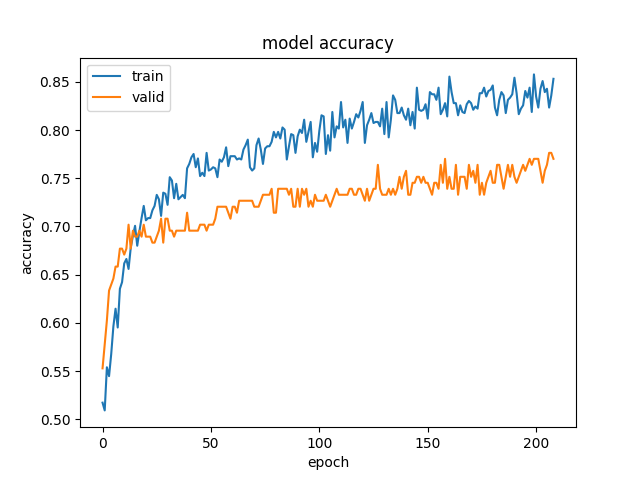
\includegraphics[width =2.5in]{images/appendice/stl/incnet/accuracy.png}} 
\subfloat[Loss]{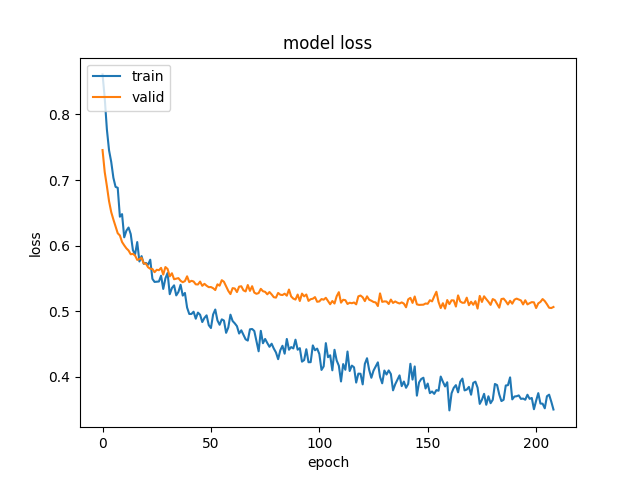
\includegraphics[width = 2.5in]{images/appendice/stl/incnet/loss.png}}\\
\caption{Training Curves for Single-Task learning model with $IncNet$. The y-axis indicates the metric fuction. The x-axis indicates the epochs of training.}
\label{incNettraining}
\end{figure}
\begin{figure}[ht]
\centering
{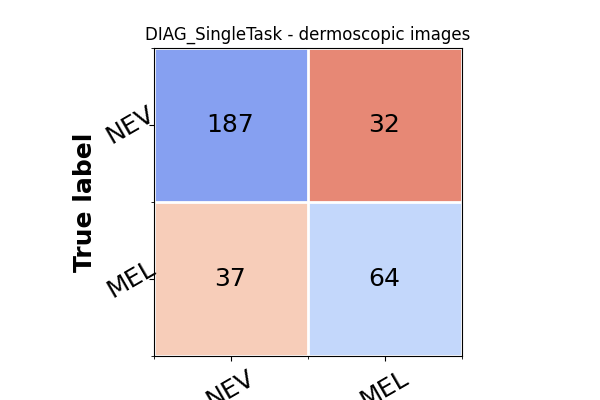
\includegraphics[width =2.5in]{images/appendice/stl/incnet/DIAG_CM_SingleTask.png}}
\caption{Confusion matrix for DIAG task using the test set prediction
from the $IncNet$ model. The y-axis indicates the ground truth labels. The x-axis indicates the model’s predicted labels. Numbers in each entry represent
the number of cases classified as such. Colors indicate the percentage of each
label in each entry, normalized by the total number of true labels.}
\label{incNetCM}
\end{figure}
\clearpage
\subsection{\texorpdfstring{\boldsymbol{$ResNet$}}{TEXT}}
\label{ResNet}
\begin{figure}[ht]
\subfloat[Accuracy]{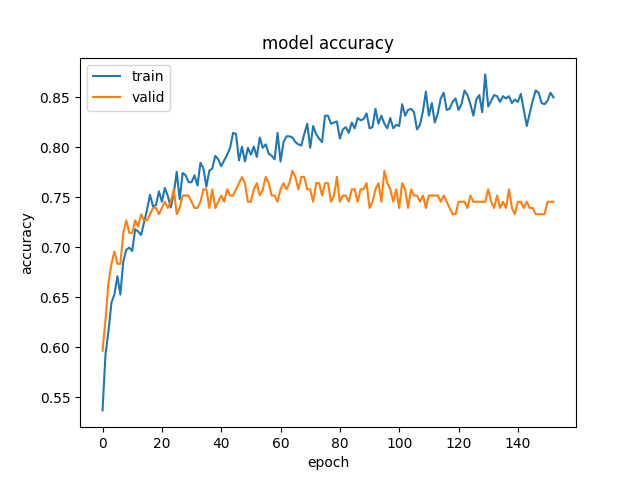
\includegraphics[width =2.5in]{images/appendice/stl/resnet/accuracy.png}} 
\subfloat[Loss]{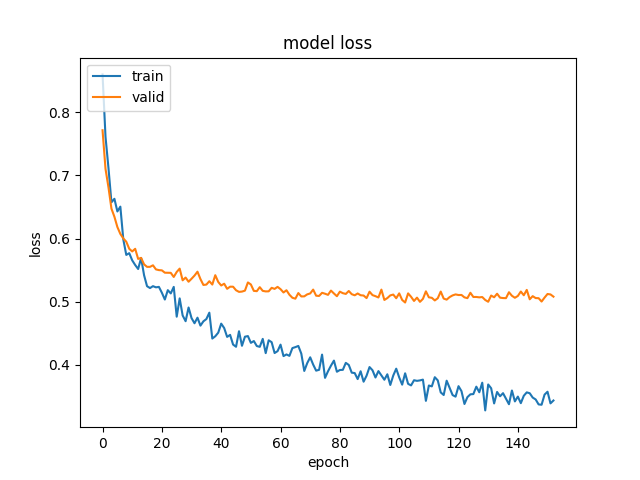
\includegraphics[width = 2.5in]{images/appendice/stl/resnet/loss.png}}\\
\caption{Training Curves for Single-Task learning model with $ResNet$. The y-axis indicates the metric fuction. The x-axis indicates the epochs of training}
\label{resNettraining}
\end{figure}
\begin{figure}[ht]
\centering
{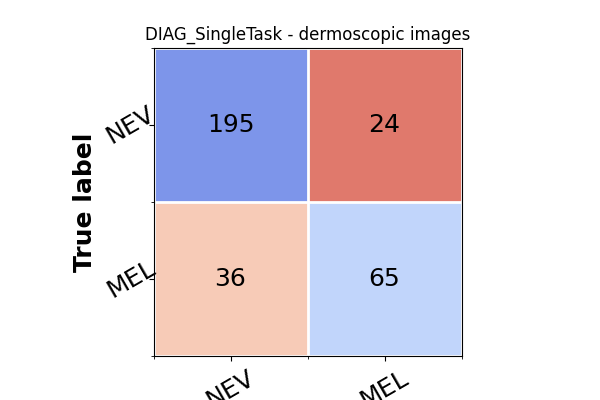
\includegraphics[width =2.5in]{images/appendice/stl/resnet/DIAG_CM_SingleTask.png}}
\caption{Confusion matrix for DIAG task using the test set prediction
from the $ResNet$ model. The y-axis indicates the ground truth labels. The x-axis indicates the model’s predicted labels. Numbers in each entry represent
the number of cases classified as such. Colors indicate the percentage of each
label in each entry, normalized by the total number of true labels.}
\label{resNetCM}
\end{figure}
\clearpage
\subsection{\texorpdfstring{\boldsymbol{$IncNet^*+L.R.$}}{TEXT}}
\begin{figure}[ht]
\centering
{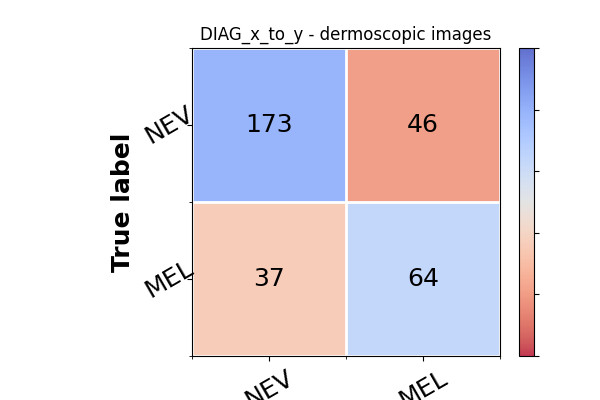
\includegraphics[width =2.5in]{images/appendice/stl/incnet+lr/DIAG_CM_x_to_y.png}}
\caption{Confusion matrix for DIAG task using the test set prediction
from the $IncNet^*+L.R.$ model. The y-axis indicates the ground truth labels. The x-axis indicates the model’s predicted labels. Numbers in each entry represent
the number of cases classified as such. Colors indicate the percentage of each
label in each entry, normalized by the total number of true labels.}
\label{incNet+lrCM}
\end{figure}

\subsection{\texorpdfstring{\boldsymbol{$ResNet^*+L.R.$}}{TEXT}}
\begin{figure}[ht]
\centering
{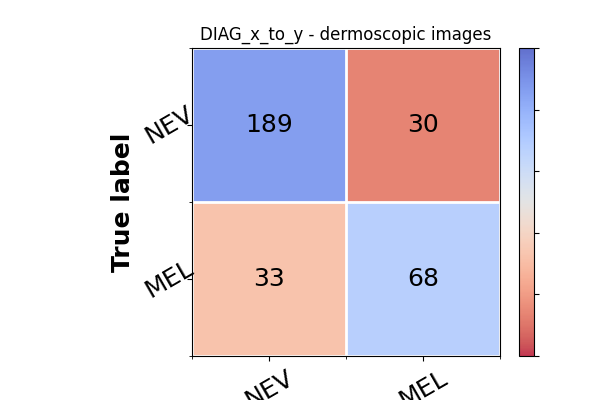
\includegraphics[width =2.5in]{images/appendice/stl/resnet+lr/DIAG_CM_x_to_y.png}}
\caption{Confusion matrix for DIAG task using the test set prediction
from the $ResNet^*+L.R.$ model. The y-axis indicates the ground truth labels. The x-axis indicates the model’s predicted labels. Numbers in each entry represent
the number of cases classified as such. Colors indicate the percentage of each
label in each entry, normalized by the total number of true labels.}
\label{resNet+lrCM}
\end{figure}



\clearpage

\section{Multi-Task Learning}

\subsection{\texorpdfstring{\boldsymbol{$IncNet_{MTL}$}}{TEXT}}
\label{MtlIncNet}
\begin{figure}[ht]
\subfloat[Accuracy]{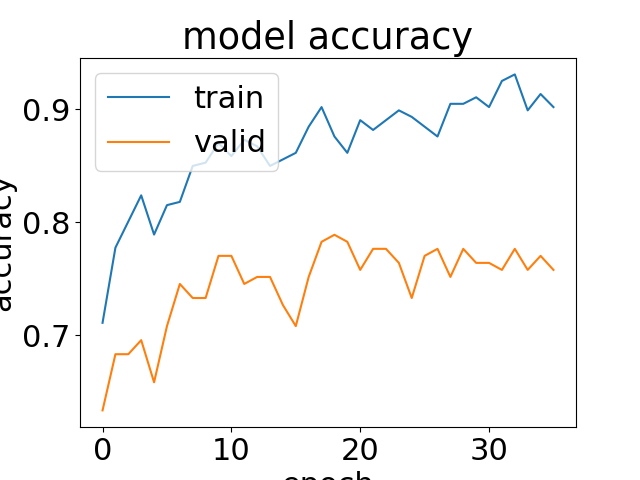
\includegraphics[width =2.5in]{images/appendice/mtl/accuracy/accuracy.png}} 
\subfloat[Loss]{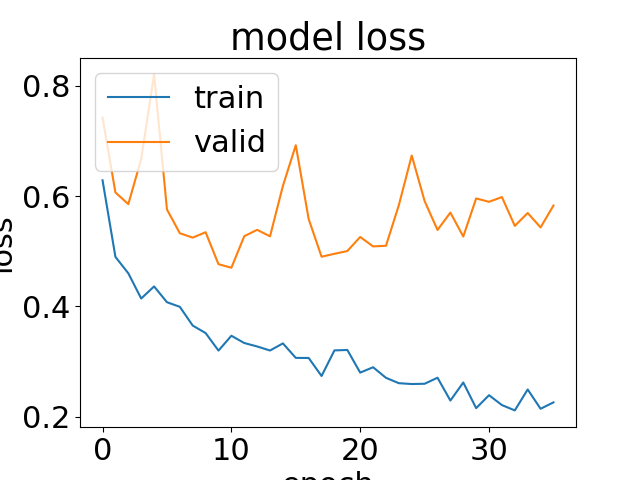
\includegraphics[width = 2.5in]{images/appendice/mtl/loss/loss.png}}

\caption{Training Curves for Multi-Task learning model with $IncNet$. The y-axis indicates the metric fuction. The x-axis indicates the epochs of training}
\label{MTLtraining}
\end{figure}

\begin{figure}[ht]
\centering
\subfloat[BWV]{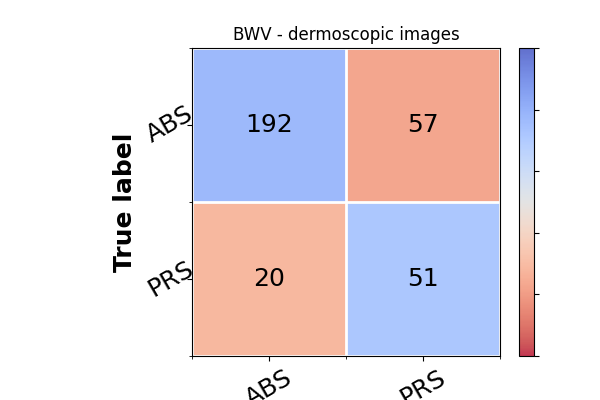
\includegraphics[width =2in]{images/appendice/mtl/CM/BWV_CM.png}} 
\subfloat[DaG]{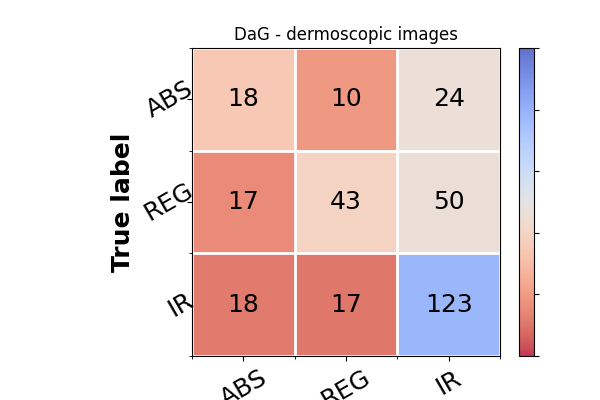
\includegraphics[width = 2in]{images/appendice/mtl/CM/DaG_CM.png}}
\subfloat[PIG]{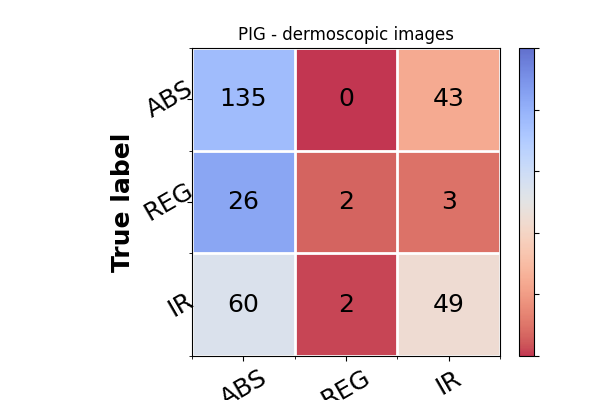
\includegraphics[width = 2in]{images/appendice/mtl/CM/PIG_CM.png}}\\
\subfloat[PN]{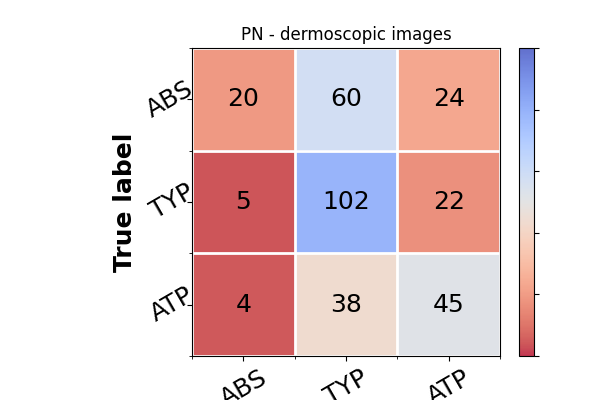
\includegraphics[width = 2in]{images/appendice/mtl/CM/PN_CM.png}} 
\subfloat[VS]{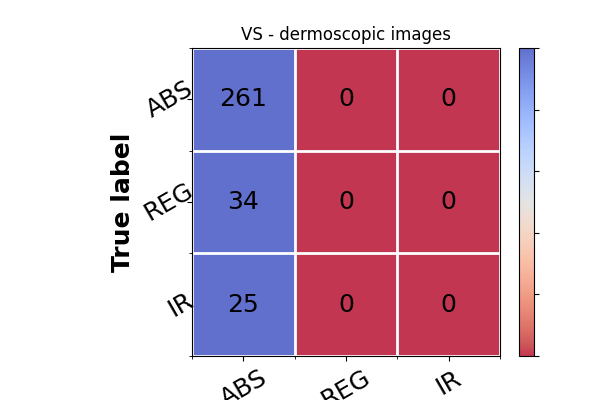
\includegraphics[width = 2in]{images/appendice/mtl/CM/VS_CM.png}}
\subfloat[STR]{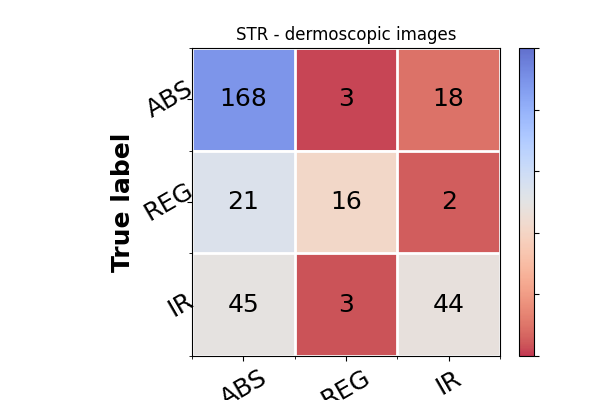
\includegraphics[width = 2in]{images/appendice/mtl/CM/STR_CM.png}}\\
\subfloat[RS]{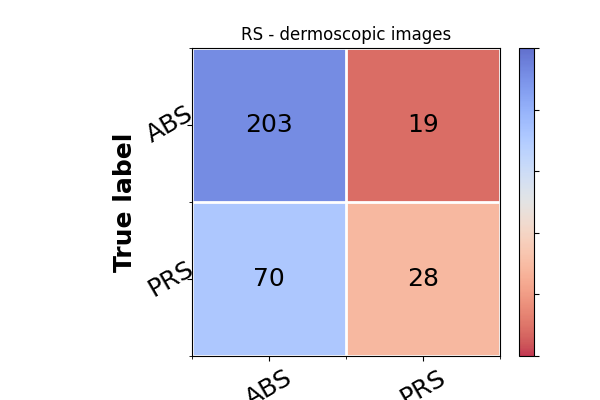
\includegraphics[width = 2in]{images/appendice/mtl/CM/RS_CM.png}} 
\caption{Confusion matrices for each concepts using the test set predictions
from the $IncNet_{MTL}$ model. The y-axis indicates the ground truth labels. The
x-axis indicates the model’s predicted labels. Numbers in each entry represent
the number of cases classified as such. Colors indicate the percentage of each
label in each entry, normalized by the total number of true labels.}
\label{CMincNetMTL}
\end{figure}

\clearpage

\subsection{\texorpdfstring{\boldsymbol{$IncNet^*_{MTL}+L.R.$}}{TEXT}}
\begin{figure}[ht]
\centering
\subfloat[BWV]{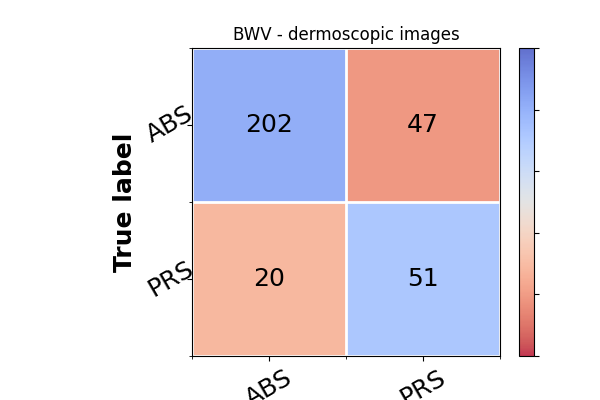
\includegraphics[width =2in]{images/appendice/incnet+lr/CM/BWV_CM.png}} 
\subfloat[DaG]{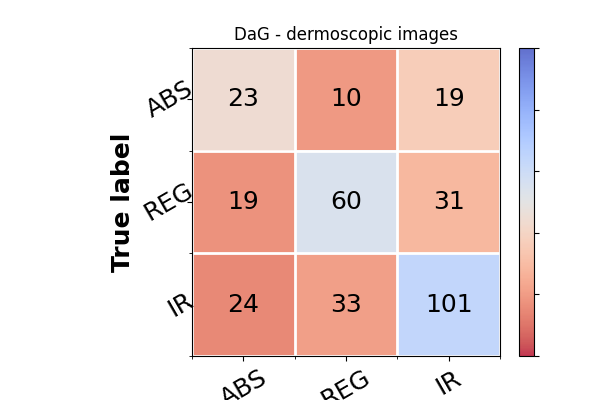
\includegraphics[width = 2in]{images/appendice/incnet+lr/CM/DaG_CM.png}}
\subfloat[PIG]{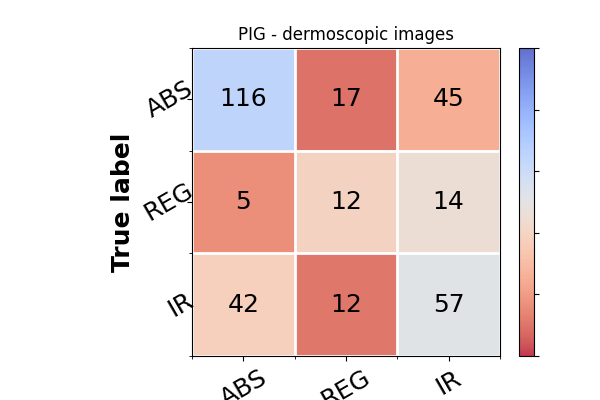
\includegraphics[width = 2in]{images/appendice/incnet+lr/CM/PIG_CM.png}}\\
\subfloat[PN]{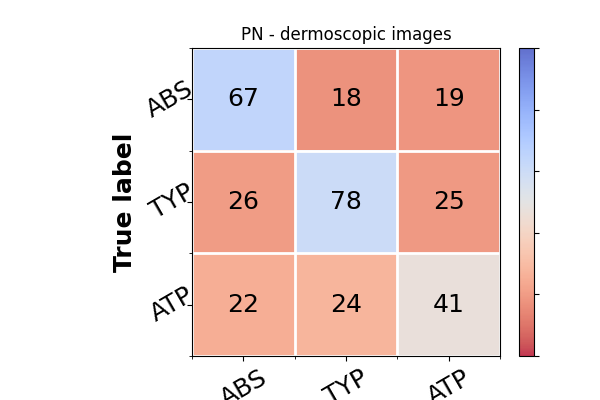
\includegraphics[width = 2in]{images/appendice/incnet+lr/CM/PN_CM.png}} 
\subfloat[VS]{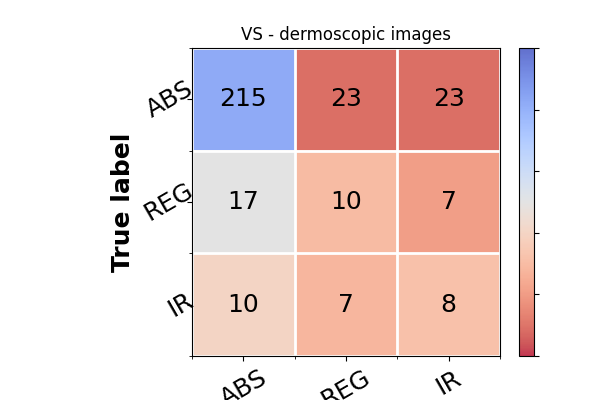
\includegraphics[width = 2in]{images/appendice/incnet+lr/CM/VS_CM.png}}
\subfloat[STR]{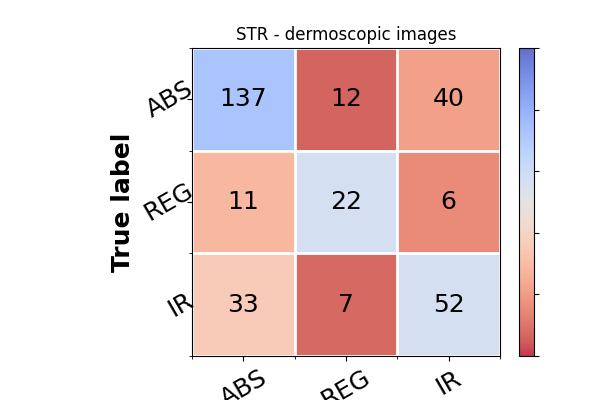
\includegraphics[width = 2in]{images/appendice/incnet+lr/CM/STR_CM.png}}\\
\subfloat[RS]{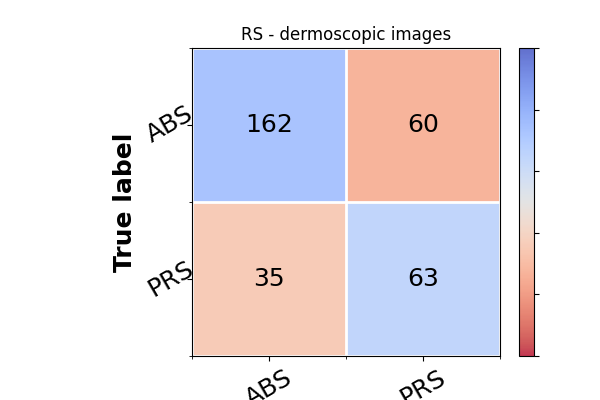
\includegraphics[width = 2in]{images/appendice/incnet+lr/CM/RS_CM.png}} 
\caption{Confusion matrices for each concepts using the test set predictions
from the $IncNet^*_{MTL}+L.R.$ model. The y-axis indicates the ground truth labels. The x-axis indicates the model’s predicted labels. Numbers in each entry represent
the number of cases classified as such. Colors indicate the percentage of each
label in each entry, normalized by the total number of true labels.}
\label{CMincNetMTLLR}
\end{figure}
\clearpage
\subsection{\texorpdfstring{\boldsymbol{$ResNet^*_{MTL}+L.R.$}}{TEXT}} 
\begin{figure}[ht]
\centering
\subfloat[BWV]{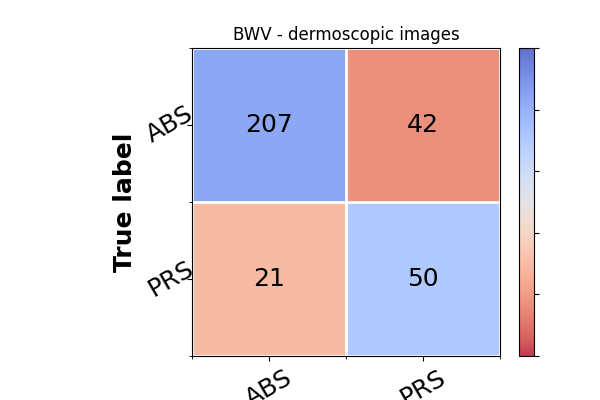
\includegraphics[width =2in]{images/appendice/resnet+lr/CM/BWV_CM.png}} 
\subfloat[DaG]{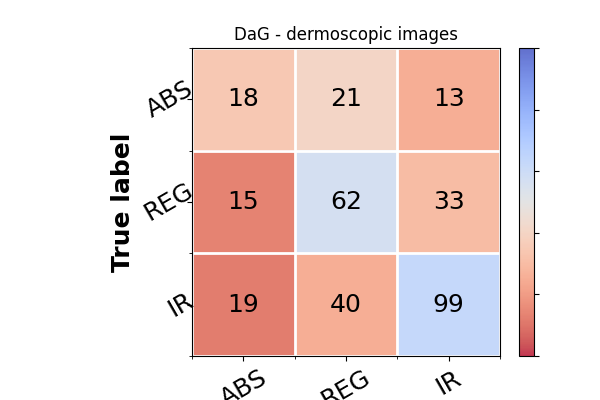
\includegraphics[width = 2in]{images/appendice/resnet+lr/CM/DaG_CM.png}}
\subfloat[PIG]{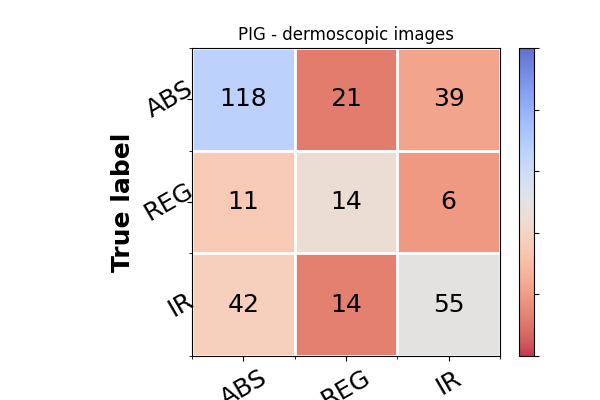
\includegraphics[width = 2in]{images/appendice/resnet+lr/CM/PIG_CM.png}}\\
\subfloat[PN]{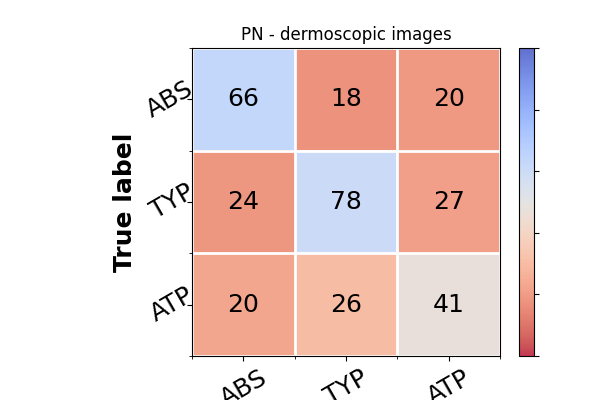
\includegraphics[width = 2in]{images/appendice/resnet+lr/CM/PN_CM.png}}
\subfloat[VS]{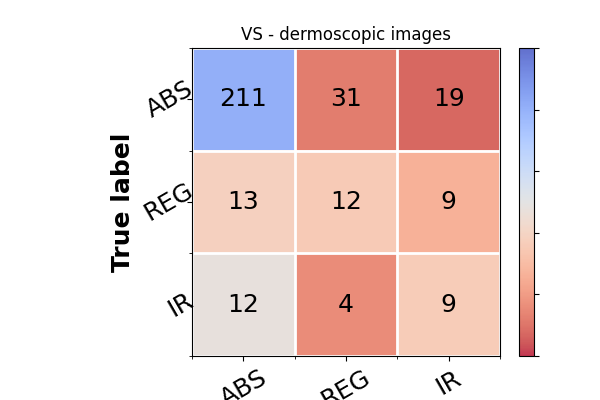
\includegraphics[width = 2in]{images/appendice/resnet+lr/CM/VS_CM.png}}
\subfloat[STR]{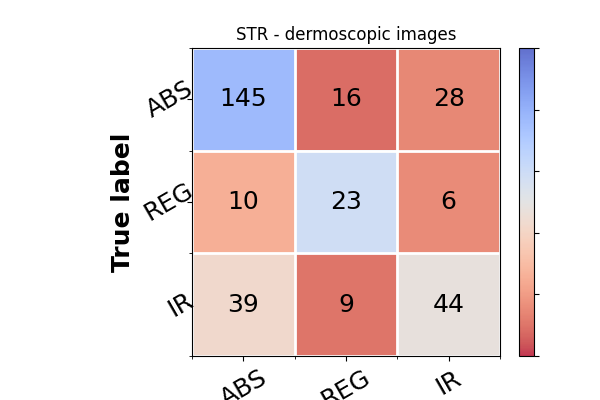
\includegraphics[width = 2in]{images/appendice/resnet+lr/CM/STR_CM.png}}\\
\subfloat[RS]{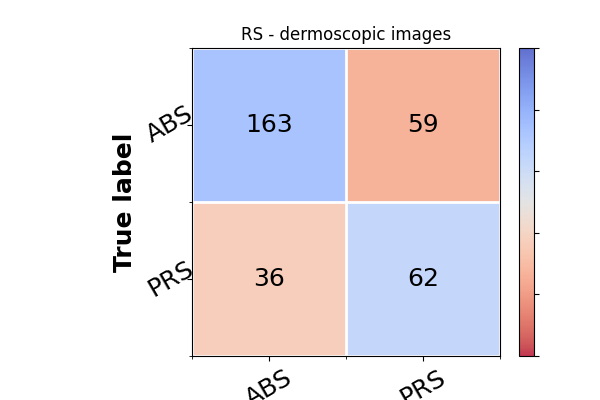
\includegraphics[width = 2in]{images/appendice/resnet+lr/CM/RS_CM.png}} 
\caption{Confusion matrices for each concepts using the test set predictions
from the $ResNet^*_{MTL}+L.R.$ model. The y-axis indicates the ground truth labels. The x-axis indicates the model’s predicted labels. Numbers in each entry represent
the number of cases classified as such. Colors indicate the percentage of each
label in each entry, normalized by the total number of true labels.}
\label{CMincNetMTLLR}
\end{figure}

\clearpage
\section{Concept-Bottleneck Models}

\subsection{\texorpdfstring{\boldsymbol{$Ind|IncNet_{MTL}$}}{TEXT}}
\begin{figure}[ht]
\centering
{\includegraphics[width =2.5in]{images/appendice/mtl/DIAG_CM_IndMod.png}}
\caption{Confusion matrix for DIAG task using the test set prediction
from the $Ind|IncNet_{MTL}$ model. The y-axis indicates the ground truth labels. The x-axis indicates the model’s predicted labels. Numbers in each entry represent
the number of cases classified as such. Colors indicate the percentage of each
label in each entry, normalized by the total number of true labels.}
\label{IndincNetCM}
\end{figure}

\subsection{\texorpdfstring{\boldsymbol{$Seq|IncNet_{MTL}$}}{TEXT}}
\begin{figure}[ht]
\centering
{\includegraphics[width =2.5in]{images/appendice/mtl/DIAG_CM_SeqMod.png}}
\caption{Confusion matrix for DIAG task using the test set prediction
from the $Seq|IncNet_{MTL}$ model. The y-axis indicates the ground truth labels. The x-axis indicates the model’s predicted labels. Numbers in each entry represent
the number of cases classified as such. Colors indicate the percentage of each
label in each entry, normalized by the total number of true labels.}
\label{SeqincNetCM}
\end{figure}
\clearpage

\subsection{\texorpdfstring{\boldsymbol{$Ind|IncNet^*_{MTL}+L.R.$}}{TEXT}}
\begin{figure}[ht]
\centering
{\includegraphics[width =2.5in]{images/appendice/incnet+lr/DIAG_CM_IndMod.png}}
\caption{Confusion matrix for DIAG task using the test set prediction
from the $Ind|IncNet^*_{MTL}+L.R.$ model. The y-axis indicates the ground truth labels. The x-axis indicates the model’s predicted labels. Numbers in each entry represent
the number of cases classified as such. Colors indicate the percentage of each
label in each entry, normalized by the total number of true labels. }
\label{IndincNet+lrCM}
\end{figure}

\subsection{\texorpdfstring{\boldsymbol{$Ind|ResNet^*_{MTL}+L.R.$}}{TEXT}}
\begin{figure}[ht]
\centering
{\includegraphics[width =2.5in]{images/appendice/resnet+lr/DIAG_CM_IndMod.png}}
\caption{Confusion matrix for DIAG task using the test set prediction
from the $Ind|ResNet^*_{MTL}+L.R.$ model. The y-axis indicates the ground truth labels. The x-axis indicates the model’s predicted labels. Numbers in each entry represent
the number of cases classified as such. Colors indicate the percentage of each
label in each entry, normalized by the total number of true labels.}
\label{IndresNet+lrCM}
\end{figure}
\clearpage

\subsection{\texorpdfstring{\boldsymbol{$Seq|IncNet^*_{MTL}+L.R.$}}{TEXT}}
\begin{figure}[ht]
\centering
{\includegraphics[width =2.5in]{images/appendice/incnet+lr/DIAG_CM_SeqMod.png}}
\caption{Confusion matrix for DIAG task using the test set prediction
from the $Seq|IncNet^*_{MTL}+L.R.$ model. The y-axis indicates the ground truth labels. The x-axis indicates the model’s predicted labels. Numbers in each entry represent
the number of cases classified as such. Colors indicate the percentage of each
label in each entry, normalized by the total number of true labels.}
\label{SeqincNet+lrCM}
\end{figure}

\subsection{\texorpdfstring{\boldsymbol{$Seq|ResNet^*_{MTL}+L.R.$}}{TEXT}}
\begin{figure}[ht]
\centering
{\includegraphics[width =2.5in]{images/appendice/resnet+lr/DIAG_CM_SeqMod.png}}
\caption{Confusion matrix for DIAG task using the test set prediction
from the $Seq|ResNet^*_{MTL}+L.R.$ model. The y-axis indicates the ground truth labels. The x-axis indicates the model’s predicted labels. Numbers in each entry represent
the number of cases classified as such. Colors indicate the percentage of each
label in each entry, normalized by the total number of true labels.}
\label{SeqresNet+lrCM}
\end{figure}
\clearpage
\section{7-pt Checklist Rule}
\begin{figure}[ht]
\centering
{\includegraphics[width =2.5in]{images/appendice/DIAG_CM_7pt_trueC.png}}
\caption{Confusion matrix for DIAG task using the test set prediction
from the 7-pt Checlist Rule. The y-axis indicates the ground truth labels. The x-axis indicates the model’s predicted labels. Numbers in each entry represent
the number of cases classified as such. Colors indicate the percentage of each
label in each entry, normalized by the total number of true labels.}
\label{7ptCm}
\end{figure}

%%%%%%%%%%%%%%%%%%%%%%%%%%%%%%%%%%%%%%%%%%%%%%%%%%%%%%%%%%%
% Back matter contents
%%%%%%%%%%%%%%%%%%%%%%%%%%%%%%%%%%%%%%%%%%%%%%%%%%%%%%%%%%%
\backmatter

%\bibliographystyle{IEEEbib}
%\bibliography{IEEEabrv,bibliografia}

\bibliographystyle{unsrt}
\bibliography{frontbackmatters/bibliography.bib}

\end{document}
